% FILE: sentiment_fgsa.tex  Version 0.0.1
% AUTHOR: Uladzimir Sidarenka

% This is a modified version of the file main.tex developed by the
% University Duisburg-Essen, Duisburg, AG Prof. Dr. G�nter T�rner
% Verena Gondek, Andy Braune, Henning Kerstan Fachbereich Mathematik
% Lotharstr. 65., 47057 Duisburg entstanden im Rahmen des
% DFG-Projektes DissOnlineTutor in Zusammenarbeit mit der
% Humboldt-Universitaet zu Berlin AG Elektronisches Publizieren Joanna
% Rycko und der DNB - Deutsche Nationalbibliothek

\chapter{Fine-Grained Sentiment Analysis}\label{chap:fgsa}

The task of fine-grained sentiment analysis (FGSA) is to automatically
recognize subjective evaluative opinions (\emph{sentiments}), holders
of these opinions (\emph{sources}), and their respective evaluated
entities (\emph{targets}) in text.  Since an accurate automatic
prediction of these elements would allow us to track public's attitude
towards literally any object (\eg{} a product, a service, or a
political decision), FGSA is traditionally considered as one of the
most attractive, necessary, but, unfortunately, also challenging
objectives in the opinion-mining field.

Researchers usually interpret this goal as a sequence labeling (SL)
objective, and address it with one of two most popular SL techniques:
conditional random fields (CRFs) or recurrent neural networks (RNNs).
The former approach represents a discriminative probabilistic
graphical model, which relies on an extensive set of hand-crafted
features, whereas the latter methods use a recursive computational
loop and learn their feature representations completely automatically.
In this chapter, we are going to evaluate each of these solutions in
detail in order to find out which of these algorithms is better suited
for the domain of German Twitter.  But before we proceed with our
experiments, we should first briefly discuss evaluation metrics that
we are going to use to estimate the quality of these systems.

%% \section{Definition of the Sentiment, Target, and Source Spans}
%% Despite some notable advances and an ongoing active research on
%% fine-grained opinion extraction, the crucial task of defining the
%% exact boundaries of sentiment spans and the spans of their respective
%% targets and sources has not been addressed in the literature with the
%% due attention yet.  Researchers typically overlook this problem,
%% leaving its solution to the discretion of their annotators
%% \cite[see][]{Wiebe:05,Klinger:13}.

%% In contrast to these works, instead of relying on rather intuitive
%% decisions of our coders, we explicitly provided a rule for determining
%% opinions' boundaries by telling the experts to assign the
%% \textsc{sentiment} label to ``\emph{minimal complete syntactic or
%%   discourse-level units that included both the target of an opinion
%%   and its actual evaluation}.''

%% % According to this instruction, during the annotation, linguists first
%% % had to identify evaluated objects (targets) in text, then find the
%% % respective evaluative expressions of these objects (usually but not
%% % necessarily polar terms), and, finally, determine the smallest
%% % syntactic components (typically noun or verb phrases) or discourse
%% % units (clauses or sentences) where both of these entities appeared
%% % together.

%% A sample annotation analyzed in compliance with this rule is shown in
%% Example~\ref{snt:fgsa:exmp:sent-anno1}:
%% \begin{example}[Annotation of a Sentiment Span]\label{snt:fgsa:exmp:sent-anno1}
%%   \upshape\sentiment{Der neue Papst gilt als
%%     bescheidener, zur\"uckgenommener Typ.}\\[0.8em]
%%   \noindent\sentiment{The new Pope is believed to be a sober, modest
%%     man.}
%% \end{example}
%% \noindent In this sentence, an expert had to label the complete
%% sentence as a sentiment, since this unit was the minimal syntactic
%% constituent which included both the object of the evaluation---``der
%% neue Papst'' (\textit{the new pope})---and the evaluation
%% itself---``bescheidener, zur\"uckgenommener Typ'' (\textit{a sober,
%%   modest man}).

%% We applied the same principles of minimality and completeness to the
%% annotation of targets and sources, requiring the main components of
%% these elements (typically nouns or verbs) to be labeled along with all
%% their syntactic dependents.  Accordingly, the correct annotation of
%% the target in the previous example had to look as follows:
%% \begin{example}[Annotation of a Target Span]\label{snt:fgsa:exmp:sent-anno2}
%%   \upshape\sentiment{\target{Der neue Papst} gilt als
%%     bescheidener, zur\"uckgenommener Typ.}\\[0.8em]
%%   \noindent\sentiment{\target{The new Pope} is believed to be a sober,
%%     modest man.}
%% \end{example}
%% \noindent with the \textsc{target} span assigned to the whole noun
%% phrase---``der neue Papst'' (\textit{the new pope})---and not only its
%% main word.

%% Similarly, source elements had to cover complete syntactic structures
%% as shown in Example~\ref{snt:fgsa:exmp:src-anno1}:
%% \begin{example}[Annotation of a Source Span]\label{snt:fgsa:exmp:src-anno1}
%%   \upshape\sentiment{Die Homosexuellenehe war f\"ur \source{den Kardinal, der jetzt Papst ist,} eine Zerst\"orung von Gottes Plan}\\[0.8em]
%%   \noindent\sentiment{For \source{the cardinal, who is the Pope now,}
%%     the same-sex marriage was a destruction of God's plan.}
%% \end{example}
%% \noindent This time, again, the whole noun phrase including the
%% dependent attributive clause---``den Kardinal, der jetzt Papst ist,''
%% (\textit{the cardinal, who is the Pope now,})---had to be labeled with
%% the \textsc{source} tag because this constituent was the only
%% \emph{minimal complete} syntactic node which encompassed both the
%% immediate holder of the opinion---``Kardinal'' \textit{cardinal}---and
%% its grammatical dependents, without including any of its parental
%% elements.

\section{Evaluation Metrics}

Because fine-grained sentiment analysis operates on \emph{spans} of
sentiment labels, which typically consist of multiple contiguous tags,
we cannot straightforwardly apply metrics that are used for evaluation
of single independent instances to this objective, as it is unclear
which instances should be measured---single tokens or complete
spans---and how partial matches should be counted in the latter case.

One possibility to estimate the quality of FGSA prediction is to
compute precision, recall, and \F{}-scores of predicted spans by using
\emph{binary-overlap} or \emph{exact-match}
metrics~\cite[see][]{Choi:06,Breck:07}.  The first method considers an
automatically labeled span as correct if it has at least one token in
common with a labeled element from the gold annotation.  The second
metric only regards an automatic span as true positive if its
boundaries are absolutely identical with the span annotated by the
human expert.  Unfortunately, both of these approaches are problematic
to a certain extent: While binary overlap might be overly optimistic,
always assigning perfect scores to automatic spans that cover the
whole sentence; exact match might, vice versa, be too drastic,
considering the whole assignment as false if only one (possibly
irrelevant) token is classified incorrectly.

Instead of relying on these measures, we decided to use a ``golden
mean'' solution proposed by \citet{Johansson:10a}, in which they
penalize predicted spans proportionally to the number of tokens whose
labels are different from the gold annotation.  More precisely, given
two sets of manually and automatically tagged spans ($\mathcal{S}$ and
$\widehat{\mathcal{S}}$, respectively), \citeauthor{Johansson:10a}
estimate the precision of automatic assignment as:
\begin{equation}\label{eq:fgsa:jmmetric}
  P(\mathcal{S}, \widehat{\mathcal{S}}) = \frac{C(\mathcal{S},
    \widehat{\mathcal{S}})}{|\widehat{\mathcal{S}}|},
\end{equation}
where $C(\mathcal{S},\widehat{\mathcal{S}})$ stands for the proportion
of overlapping tokens across all pairs of manually ($s_i$) and
automatically ($s_j$) annotated spans:
\begin{equation*}
  C(\mathcal{S}, \widehat{\mathcal{S}}) = \sum_{s_i \in
    \mathcal{S}}\sum_{s_j \in \widehat{\mathcal{S}}}c(s_i, s_j),
\end{equation*}
and the $|\widehat{\mathcal{S}}|$ term denotes the total number of
spans automatically labeled with the given tag.

Similarly, the recall of this assignment is estimated as:
\begin{equation*}
  R(\mathcal{S}, \widehat{\mathcal{S}}) = \frac{C(\mathcal{S},
    \widehat{\mathcal{S}})}{|\mathcal{S}|}.
\end{equation*}

Using these two values, one can normally compute the \F{}-measure as:
\begin{equation*}
  F_1 = 2\times\frac{P \times R}{P + R}.
\end{equation*}

Because this estimation adequately accommodates both extrema of
automatic annotation (too long and too short spans) and also penalizes
erroneous labels, we will rely on this measure throughout our
subsequent experiments.

\section{Data Preparation}\label{snt:fgsa:subsec:data}

In order to evaluate CRFs and RNNs on our dataset, we split the
complete corpus annotated by the second annotator, which we will
henceforth consider as gold standard in all subsequent experiments,
into three parts, using 70\% of it for training, 10\% as development
data, and the remaining 20\% as a test set.  We tokenized all tweets
with the same adjusted version of Potts' tokenizer that we used
previously while creating the initial corpus files, and preprocessed
these microblogs with the rule-based normalization pipeline of
\citet{Sidarenka:13}.  In this procedure, we:
\begin{itemize}
\item \emph{unified Twitter-specific phenomena} such as @-mentions,
  hyperlinks, and e-mail addresses by replacing these entities with
  special tokens that represented their semantic classes (\eg{}
  ``\%Username'' for @-mentions, ``\%URI'' for hyperlinks).  We
  removed these elements from the input, if they were grammatically
  independent from the rest of the tweet and did not play a potential
  role for the expression of sentiments (\eg{} we stripped off all
  retweet mentions and hyperlinks appearing at the very end of the
  microblog if they were not preceded by a preposition).  Furthermore,
  we substituted all emoticons with special placeholders representing
  their semantic orientation (\eg{} \smiley{} $\rightarrow$
  ``\%PosSmiley,'' \frownie{} $\rightarrow$ ``\%NegSmiley,''
  \texttt{:-O} $\rightarrow$ ``\%Smiley''), and removed the hash sign
  (\#) from all hashtags (\eg{} ``\#gl\"ucklich'' $\rightarrow$
  ``gl\"ucklich'');

\item In addition to this, we \emph{restored frequent misspellings}
  (\eg{} ``zuguckn'' $\rightarrow$ ``zugucken'' [\emph{to watch}],
  ``Tach'' $\rightarrow$ ``Tag'' [\emph{day}]), using a set of
  manually-defined heuristic rules;

\item and, finally, \emph{replaced frequent slang terms and
  abbrebiations with their standard-language equivalents} (\eg{} ``n
  bissl'' $\rightarrow$ ``ein bisschen'' [\emph{a bit of}], ``iwie''
  $\rightarrow$ ``irgendwie'' [\emph{somehow}], ``nix'' $\rightarrow$
  ``nichts'' [\emph{nothing}]).
\end{itemize}

%% During the normalization, Twitter-specific phenomena like @-mentions,
%% retweets, and URIs that were not syntactically integrated in any
%% sentence of the message were removed from the tweets and those
%% elements which played an integral syntactic role were replaced with
%% the special artificial tokens \%User, \%Link etc.  Emoticons like :-),
%% \smiley{}, \frownie{} etc. were also replaced with the placeholders
%% \%PosSmiley, \%NegSmiley, or simply \%Smiley depending on their prior
%% polarity.  Furthemore, out-of-vocabulary words which could be
%% converted to in-vocabulary terms with a pre-defined set of
%% transformations were also normalized.
Afterwards, we labeled all normalized sentences with part-of-speech
tags using \textsc{TreeTagger}\footnote{In particular, we used
  \textsc{TreeTagger} Version~3.2 with the German parameter file
  UTF-8.}~\cite{Schmid:95}, and parsed them with the \textsc{Mate}
dependency parser\footnote{We used \textsc{Mate} Version \texttt{3.61}
  with the German parameter model 3.6.}
\cite{Bohnet:13}.\footnote{The choice of these tools was motivated by
  their better results in our evaluation study, which we conducted
  while working on the normalization module \cite{Sidarenka:13}.}
Finally, since \texttt{MMAX2} did not provide a straightforward
support for character offsets of annotated tokens and because
automatically tokenized data could disagree with the original corpus
tokenization, we aligned manual annotation with automatically split
words with the help of the Needleman-Wunsch
algorithm~\cite{Needleman:70}.

\section{Conditional Random Fields}

The first method that we evaluated using the obtained data was
conditional random fields.  First introduced by \citet{Lafferty:01},
CRFs have rapidly grown in popularity, turning into one of the most
widely used probabilistic frameworks, which was dominating the NLP
field for almost a decade.

The main reasons for the success of this model are:
\begin{enumerate}[1)]
\item the \emph{structural nature} of CRFs, which, in contrast to
  single-entity classifiers, such as logistic regression or SVM, make
  their predictions over structured input, trying to find the most
  likely label assignment to the whole structure (typically a chain or
  a tree) and not only its individual elements;
\item the \emph{discriminative power} of this framework, which, in
  contrast to generative probabilistic models such as HMMs
  \cite{Rabiner:86}, optimizes conditional probability
  $P(\boldsymbol{Y}|\boldsymbol{X})$ instead of joint distribution
  $P(\boldsymbol{X},\boldsymbol{Y})$ and consequently can efficiently
  deal with overlapping and correlated features;
%% \begin{example}[Overlapping and Correlated Features]
%%   In order to demonstrate the different effects of correlated and
%%   overlapping features on generative and discriminative models, let us
%%   go through an example where we need to predict whether a tweet
%%   mentioning ``Merkel'' and ``Steinmeier'' is about the Christian
%%   Democratic Union (\texttt{CDU}) or Social Democratic Party of
%%   Germany (\texttt{SPD}).

%%   As features for this task, we will use lexical unigrams appearing in
%%   the training data.  Assuming that our training set consists of three
%%   messages mentioning ``Merkel'' and one microblog mentioning
%%   ``Steinmeier'' which are labeled as \texttt{CDU}, plus one tweet
%%   mentioning ``Merkel'' and three posts mentioning ``Steinmeier''
%%   which are annotated as \texttt{SPD}, the generative Na\"{i}ve Bayes
%%   model would estimate the probability of the two competing classes
%%   as:
%%   \begin{align*}
%%     P(\mathbf{x}, CDU) =& P(\textrm{Merkel},\textrm{Steinmeier}|CDU)\times P(CDU)\\
%%     =& P(\textrm{Merkel}|CDU)\times P(\textrm{Steinmeier}|CDU) \times P(CDU)\\
%%     =&\frac{3}{4}\times\frac{1}{4}\times\frac{4}{8}\approx 0.0938\\
%%     P(\mathbf{x}, SPD) =& P(\textrm{Merkel},\textrm{Steinmeier}|SPD)\times P(SPD)\\
%%     =& P(\textrm{Merkel}|SPD)\times P(\textrm{Steinmeier}|SPD) \times P(SPD)\\
%%     =&\frac{1}{4}\times\frac{3}{4}\times\frac{4}{8}\approx 0.0938.\\
%%   \end{align*}
%%   After normalizing these probabilities, we would get equal 50\%
%%   chances for each of the parties, which is fair regarding the token
%%   distribution in our corpus.  However, if we replace ``Merkel'' with
%%   ``von der Leyen'' both in the training data and test example, and
%%   rerun this experiment once again, the probability would get
%%   significantly skewed towards the CDU class:
%%   \begin{align*}
%%     P(\mathbf{x}, CDU) =& P(\textrm{von},\textrm{der},\textrm{Leyen},\textrm{Steinmeier}|CDU)\times P(CDU)\\
%%     =& P(\textrm{von}|CDU)\times P(\textrm{der}|CDU)\times P(\textrm{Leyen}|CDU)\\
%%     &\times P(\textrm{Steinmeier}|CDU) \times P(CDU)\\
%%     =&\frac{3}{4}\times\frac{3}{4}\times\frac{3}{4}\times\frac{1}{4}\times\frac{4}{8}\approx 0.0527\\
%%     P(\mathbf{x}, SPD) =& P(\textrm{von},\textrm{der},\textrm{Leyen},\textrm{Steinmeier}|SPD)\times P(SPD)\\
%%     =& P(\textrm{von}|SPD)\times P(\textrm{der}|SPD)\times P(\textrm{Leyen}|SPD)\\
%%     &\times P(\textrm{Steinmeier}|SPD) \times P(SPD)\\
%%     =&\frac{1}{4}\times\frac{1}{4}\times\frac{1}{4}\times\frac{3}{4}\times\frac{4}{8}\approx 0.0059,\\
%%   \end{align*}
%%   which, after normalization, would result in 90\% chances for
%%   \texttt{CDU}, and a 10\% score for \texttt{SPD}, even though we only
%%   changed the name of the politician.

%%   A different situation can be observed with discriminative models
%%   such as maximum entropy classifier: Instead of optimizing the joint
%%   distribution $P(\mathbf{x}, y)$ as it is done in the generative
%%   frameworks, discriminative systems seek to optimize the conditional
%%   likelihood $P(y|\mathbf{x})$ by maximizing the total probability of
%%   the training set $\sum_{i=1}^N\log P(y_i|\mathbf{x}_i, \mathbf{w})$.
%%   This probability is usually estimated using the sigmoid function
%%   $\frac{1}{1 + e^{-(\mathbf{x}_i, \mathbf{w})}}$, where
%%   $\mathbf{x}_i$ denotes the input features of the $i$-th training
%%   instance, and the vector $\mathbf{w}$ stands for the respective
%%   weights of these features.  By optimizing this function using
%%   gradient descent, we will arrive at the optimal solution
%%   $w_1 \approx 0.5$ for the feature ``Merkel'' and $w_2 \approx -0.5$
%%   for the feature ``Steinmeier'' for the first example, which would
%%   again result in equal 50\% chances for both classes.  In the second
%%   example, however, all three features ``von,'' ``der,'' and ``Leyen''
%%   would get an equal weight of $\approx 0.3$, and the ``Steinmeier''
%%   feature would receive a coefficient of $\approx -0.4$, which would
%%   result in 60\% probability for the test message being about the CDU,
%%   and 40\% that the tweet is about the SPD.  Even though this still
%%   means a slight skewness towards \texttt{CDU}; this time, the effect
%%   of correlated features is much less dramatic than in the generative
%%   case.
%% \end{example}
\item and, finally, the \emph{avoidance of the label bias problem},
  which other discriminative classifiers, such as maximum entropy
  Markov networks~\cite{McCallum:00}, are known to be susceptible to.
  \begin{example}[Label Bias Problem]
    The label bias problem arises in the cases where a locally optimal
    decision outweighs globally superior solutions.  Consider, for
    example, the sentence ``Aber gerade Erwachsene haben damit
    Schwierigkeiten.'' (\textit{But especially adults have
      difficulties with it.}), for which we need to compute the most
    probable sequence of part-of-speech tags.

    \begin{center}
      \begin{tikzpicture}[node distance=5cm]
        \tikzstyle{tag}=[circle split,draw=gray!50,%
          minimum size=2.5em,inner ysep=2,inner xsep=0,%
          circle split part fill={yellow!20,blue!30}]
      \tikzstyle{word}=[draw=none,inner sep=10pt]

      \node[word] (A) at (1, 1) {Aber};
      \node[tag] (B) at (1, 3) {\footnotesize KON \nodepart{lower} 1.};
      \node[word] (D) at (3, 1) {gerade};
      \node[tag] (E) at (3, 2) {\footnotesize ADJA \nodepart{lower} .5};
      \node[tag] (F) at (3, 4) {\footnotesize ADV \nodepart{lower} .5} ;
      \node[word] (G) at (7, 1) {Erwachsene};
      \node[tag] (I) at (7,2) {\footnotesize ADJA \nodepart{lower} .5} ;
      \node[tag] (H) at (7,4) {\footnotesize NN \nodepart{lower} .5};
      \node[word] (J) at (9,1) {haben};
      \node[tag] (K) at (9,3) {\footnotesize VA \nodepart{lower}\small 1.};
      \node[word] (J) at (11,1) {\ldots};

      \path [-] (B) edge node[below] {$.5$} (E);
      \path [-] (B) edge node[above] {$.5$} (F);

      \path [-] (E) edge node[below] {$.3$} (I);
      \path [-] (E) edge node[below left=0.4] {$.7$} (H);
      \path [-] (F) edge node[above left=0.4] {$.8$} (I);
      \path [-] (F) edge node[above] {$.2$} (H);

      \path [-] (I) edge node[below] {$.1$} (K);
      \path [-] (H) edge node[above] {$.9$} (K);
    \end{tikzpicture}
    \captionof{figure}{Example of a CRF graph}\label{fig:snt:memm-crf}
    \end{center}
    Using features weights shown in Figure~\ref{fig:snt:memm-crf}, we
    will first estimate the probability of the correct label sequence
    for the initial part of this sentence using the Maximum Entropy
    Markov Model (MEMM)---the predecessor of the Conditional Random
    Fields.  According to the MEMM's definition, the probability of
    correct labeling ($KON-ADV-NN-VA$) is equal to:
    \begin{align*}
      P(KON, ADV, NN, VA) &= P(KON)\times P(ADV|KON)\\
      &\times P(NN|ADV)\times P(VA|NN)\\
      &=\frac{\exp(1)}{\exp(1)}\times\frac{\exp(0.5 + 0.5)}{\exp(0.5 + 0.5) + \exp(0.5 + 0.5)}\\%
      &\times\frac{\exp(0.2 + 0.5)}{\exp(0.2 + 0.5) + \exp(0.8 + 0.5)}\\
      &\times\frac{\exp(0.9 + 1.)}{\exp(0.9 + 1.)} \approx 0.177
    \end{align*}
    At the same time, the probability of the wrong variant
    ($KON-ADV-ADJA-VA$) amounts to $\approx$ 0.323 and will therefore
    be preferred by the automatic tagger.

    A different situation is observed with CRFs, where the normalizing
    factor in the denominator is computed over the whole input
    sequence without factorizing into individual terms for each
    transition as it is done in MEMM\@.  This way, the probability of
    correct labels will run up to:
    \begin{align*}
      P(KON, ADV, NN, VA) =& P(KON)\times
      P(ADV|KON)\times P(NN|ADV)\\
      &\times P(VA|NN)\\ =&\frac{\exp(1 + 0.5
        \times 3 + 0.2 + 0.9 + 1)}{Z} \approx 0.252,
    \end{align*}
    where $Z = \exp(1 + 0.5 \times 3 + 0.2 + 0.9 + 1) + \exp(1 + 0.5
    \times 3 + 0.8 + 0.1 + 1) + \exp(1 + 0.5 \times 3 + 0.7 + 0.9 + 1)
    + \exp(1 + 0.5 \times 3 + 0.3 + 0.1 + 1)$ is the total score of
    all possible label assignments; the incorrect alternative
    ($KON-ADV-ADJA-VA$), however, will get a probability score of
    $\approx$ 0.207, which is less than the score of the correct
    labeling.
  \end{example}
\end{enumerate}

\paragraph{Training.}

CRFs have these useful properties due to a neatly formulated objective
function in which they seek to optimize the global log-likelihood of
gold labels $\mathbf{Y}$ conditioned on training data $\mathbf{X}$.
In particular, given a set of training instances $\mathcal{D} =
\{(\mathbf{x}^{(n)}, \mathbf{y}^{(n)})\}_{n=1}^N$, where
$\mathbf{x}^{(n)}$ stands for the covariates of the $n$-th instance,
and $\mathbf{y}^{(n)}$ denotes its respective gold labels, CRFs try to
find feature coefficients $\mathbf{w}$ that maximize the
log-probabilities $\ell$ of $\mathbf{y}^{(i)}$ given
$\mathbf{x}^{(i)}$ over the whole corpus:
\begin{equation}\label{snt:fgsa:eq:crf-w}
  \mathbf{w} = \argmax_{\mathbf{w}}\sum_{n=1}^N\ell
  \left(\mathbf{y}^{(n)}|\mathbf{x}^{(n)}\right).
\end{equation}
The log-likelihood $\ell(\mathbf{y}^{(n)}|\mathbf{x}^{(n)})$ in this
equation is commonly estimated as the logarithm of globally (\ie{}
w.r.t\@. to the whole instance) normalized softmax function:
\begin{equation}\label{snt:fgsa:eq:crf-ell}
  \ell\left(\mathbf{y}^{(n)}|\mathbf{x}^{(n)}\right) =
  \ln\left(P(\mathbf{y}^{(n)}|\mathbf{x}^{(n)})\right) =
  \ln\left(\frac{ \exp\left(\sum_{m=1}^{M}\sum_{j}w_{j} \cdot f_j(x_{m},
    y_{m-1}, y_{m})\right)}{Z}\right),
\end{equation}
in which $M$ means the length of the $n$-th training example;
$f_j(x_{m}, y_{m-1}, y_{m})$ denotes the value of the $j$-th feature
function $f$ at position $m$; $w_j$ represents the corresponding
weight of this feature; and $Z$ is a normalization factor calculated
over all possible label assignments:
\begin{equation*}
  Z \defeq
  \sum_{y'\in\mathcal{Y},y''\in\mathcal{Y}}\exp\left(\sum_{m=1}^{M}\sum_{j}w_{j}
  \cdot f_j(x_{m}, y'_{m-1}, y''_{m})\right).
\end{equation*}
Since this normalizing term appears in the denominator and couples
together all feature weights that need to be optimized, it becomes
prohibitively expensive to find the best solution to
Equation~\ref{snt:fgsa:eq:crf-w} analytically, with a single shot.  A
possible remedy to this problem is to resort to other optimization
techniques, such as gradient descent, where feature weights are
successively changed in the direction of their gradient until they
reach the minimum of the loss function.

From Equation~\ref{snt:fgsa:eq:crf-ell}, we can see that the partial
derivative of log-likelihood w.r.t\@. a single feature weight $w_j$ is:
\begin{equation*}
  \frac{\partial}{\partial w_j}\ell =%
  \sum_{n=1}^N\sum_{m=1}^{M}f_j(x_{m}, y_{m-1}, y_{m}) -%
  \sum_{n=1}^N\sum_{m=1}^{M}\sum_{y'\in\mathcal{Y},y''\in\mathcal{Y}}f_j(x_{m},%
  y'_{m-1}, y''_{m})P(y',y''|\mathbf{x}^{(n)}),
\end{equation*}
which, after dividing both parts of the equation by the constant term
$N$ (the size of the corpus) can be transformed into:
\begin{equation*}
  \frac{1}{N}\frac{\partial}{\partial w_j}\ell = \E[f_j(\mathbf{x},
  \mathbf{y})] - \E_{\mathbf{w}}[f_j(\mathbf{x}, \mathbf{y})],
\end{equation*}
where the first term ($\E[f_j(\mathbf{x}, \mathbf{y})]$) is the
expectation of feature $f_j$ under empirical distribution, and the
second term ($\E_{\mathbf{w}}[f_j(\mathbf{x}, \mathbf{y})]$) is the
same expectation under model's parameters $\mathbf{w}$.  In other
words, the optimal solution to the log-likelihood objective in
Equation~\ref{snt:fgsa:eq:crf-ell} is achieved when model's
expectation of features matches their (true) empirical expectation on
the corpus.

The marginal probabilities of these features, which are required for
computing their expectations, can be estimated dynamically using the
forward-backward (FB) algorithm~\cite{Rabiner:90}, which is a
particular case of the more general belief-propagation
method~\cite[see][p.~81]{Barber:12}.

The only modification that one usually makes to
Equation~\ref{snt:fgsa:eq:crf-w} in practice, before applying it the
the provided training set, is the addition of so-called
\emph{regularization terms} (L1 and L2), which penalize excessively
high feature weights, thus preventing the model from overfitting the
training data, \ie{} we no longer seek feature weights that simply
maximize the probability of observed data, but we also want these
weights to be as small as possible:
\begin{equation}\label{snt:fgsa:eq:crf-w-regularization}
\mathbf{w} = \argmax_{\mathbf{w}}\sum_{n=1}^N\ell
\left(\mathbf{y}^{(n)}|\mathbf{x}^{(n)}\right) -
\lambda_1\lVert\mathbf{w}\rVert_1 - \lambda_2\lVert\mathbf{w}\rVert_2,
\end{equation}
where $\lambda_1$ and $\lambda_2$ are manually set hyper-parameters,
which control the amount of penalty that we want impose on the L1 and
L2 norms of the weights.

In our experiments, we also adopted this enhanced objective, picking
hyper-parameter values that yielded the best results on the held-out
development set.  Furthermore, in order to reduce the noise that is
typically introduced by rare, sporadic features, we only optimized the
weights of features that occurred two or more times in the training
corpus, ignoring all singleton attributes from these data.

\paragraph{Inference.}

Once optimal feature weights have been learned, one can
unproblematically compute the most likely label assignment for a new
instance by using the Viterbi algorithm~\cite{Viterbi:67}, which
effectively corresponds to the forward pass of the FB method with the
summation over the alternative preceding states replaced by the
maximum operator (hence the other name for this algorithm,
``max-product'').

\paragraph{Features.}

A crucial component that accounts for a huge part of the success (or
failure) of CRFs is features that are provided to this classifier as
input.

Traditionally, feature functions in CRFs are divided into transition-
and state-based ones.  Transition features represent real- or
binary-valued functions $f(\mathbf{x}, y'', y')\rightarrow\mathbb{R}$
associated with some data predicate
$\phi(\mathbf{x})\rightarrow\mathbb{R}$ and two labels $y''$
(typically the label of the previous token) and $y'$ (usually the
label of the current word).  The value of this function at position
$m$ in sequence $\mathbf{x}$ is then defined as:
\begin{equation*}
  f(\mathbf{x}_m, y'', y') = \begin{cases} \phi(\mathbf{x}_m), &
    \mbox{if } \mathbf{y}_{m-1} = y''\mbox{ and }\mathbf{y}_{m} =
    y'\\ 0, & \mbox{otherwise;}
  \end{cases}
\end{equation*}
where predicate~$\phi$ usually represents a simple unit function:
$\phi(\mathbf{x}_m)\mapsto 1$, $\forall\mathbf{x}_m$.

In contrast to ternary transition features, state attributes are
typically associated with binary predicates, whose output depends on
the input data at the given position and label $y'$ at the respective
state:
\begin{equation*}
  f(\mathbf{x}_m, y') = \begin{cases} \phi(\mathbf{x}_m), & \mbox{if }
    \mathbf{y}_{m} = y'\\ 0, & \mbox{otherwise.}
  \end{cases}
\end{equation*}
This time, predicate~$\phi$ is usually much more sophisticated and
reflects various properties of the input, such as whether the current
token is capitalized or whether it begins with a specific prefix or
ends with a certain suffix.  This type of features commonly accounts
for the overwhelming majority of all attributes in CRFs.

As state attributes in our experiments, we used the following
features, which, for simplicity, are listed in groups:
\begin{itemize}
\item\emph{formal}, which included the initial three characters of
  each token (\eg{} $\phi_{abc}(\mathbf{x}_m) = 1\mbox{ if
  }\mathbf{x}_m\sim\mbox{ /\textasciicircum{}abc/ else } 0$), its last
  three characters, and the spelling class of that word (\eg{}
  alphanumeric, digit, or punctuation);

\item\emph{morphological}, which encompassed part-of-speech tags of
  analyzed tokens, grammatical case and gender of inflectable PoS
  types, degree of comparison for adjectives, as well as mood, tense,
  and person forms for verbs;

\item\emph{lexical}, which comprised the actual lemma and form of the
  analyzed token (using one-hot encoding), its polarity class
  (positive, negative, or neutral), which we obtained from the Zurich
  Polarity Lexicon~\cite{Clematide:10};

\item and, finally, \emph{syntactic} features, which reflected the
  dependency relation via which token $x_m$ was connected to its
  parent.  In addition to this, we also used two binary attributes
  that showed whether the previous token in the sentence was the
  parent (first feature) or a child (second feature) of the current
  word.  Apart from that, we devised two more features, one of which
  encoded the dependency relation of the previous token in the
  sentence to its parent + the dependency relation of the current
  token to its ancestor; another feature reflected the dependency link
  of the next token + the dependency relation of the current token to
  its parent.
\end{itemize}

Besides the above attributes, we also introduced a set of complex
\emph{lexico-syntactic} features, which simultaneously reflected
several semantic and syntactic traits.  These were:
\begin{itemize}
\item the lemma of the syntactic parent;
\item the part-of-speech tag and polarity class of the grandparent in
  the syntactic tree;
\item the lemma of the child node + the dependency relation between
  the current token and its child;
\item the PoS tag of the child node + its dependency relation + the
  PoS tag of the current token;
\item the lemma of the child node + its dependency relation + the
  lemma of the current token;
\item the overall polarity of syntactic children, which was computed
  by summing up the polarity scores of all immediate dependents, and
  checking whether the resulting value was greater, less than, or
  equal to zero.\footnote{We again used the Zurich Polarity Lexicon
    of~\citet{Clematide:10} for computing these scores.}
\end{itemize}

\paragraph{Results.}

The results of our experiments are shown in
Table~\ref{snt-fgsa:tbl:crf-res}.  As we can see from the table, with
the given set of features, CRF can perfectly well fit the training
data, achieving a macro-averaged \F-score of~0.904.  This model,
however, can only partially generalize to unseen messages, where its
macro-\F{} reaches merely~0.287, despite the fact that the size of the
training corpus is almost 3.5 times bigger than the size of the test
set (5,616 versus 1,584 tweets).

%% There are 5,616 training tweets, 792 development and 1,584 test microblogs.
%% ./scripts/cmp_features --min-cnt=2 lingtmp/sentiment/crf/train/ lingtmp/sentiment/crf/devtest/
%% Features in first dataset: 34597
%% Features in second dataset: 28579
%% Common features: 11317
%% Total features: 51859

%% ./scripts/cmp_features --min-cnt=2 lingtmp/sentiment/crf/train/ lingtmp/sentiment/crf/test/
%% Features in first dataset: 34597
%% Features in second dataset: 49626
%% Common features: 15440
%% Total features: 68783

%% Another notable tendency that can be observed both on the training and
%% test sets, is that the recall of the CRF system is generally lower
%% than its precision.  This again can be attributed to the high variance
%% of the classifier.

\begin{table*}
  \begin{center}
    \bgroup\setlength\tabcolsep{0.1\tabcolsep}\scriptsize
    \begin{tabular}{p{0.162\columnwidth} % first columm
        *{9}{>{\centering\arraybackslash}p{0.074\columnwidth}} % next nine columns
        *{1}{>{\centering\arraybackslash}p{0.136\columnwidth}}} % last two columns
      \toprule
      \multirow{2}*{\bfseries Data Set} & \multicolumn{3}{c}{\bfseries Sentiment} & %
      \multicolumn{3}{c}{\bfseries Source} & %
      \multicolumn{3}{c}{\bfseries Target} & %
      \multirow{2}{0.136\columnwidth}{\bfseries\centering Macro\newline \F{}}\\\cmidrule(lr){2-4}\cmidrule(lr){5-7}\cmidrule(lr){8-10}

      & Precision & Recall & \F{} & %
      Precision & Recall & \F{} & %
      Precision & Recall & \F{} &\\\midrule

      Training Set & 0.949 & 0.908 & 0.928 & 0.903 & 0.87 & 0.886 & %
      0.933 & 0.865 & 0.898 & 0.904\\
      Test Set & 0.37 & 0.28 & 0.319 & 0.305 & 0.244 & 0.271 & 0.304 & %
      0.244 & 0.271 & 0.287\\\bottomrule
    \end{tabular}
    \egroup{}
    \caption{Results of fine-grained sentiment analysis with the
      first-order linear-chain CRFs}\label{snt-fgsa:tbl:crf-res}
  \end{center}
\end{table*}

\subsection{Feature Analysis}

To estimate the effect of different features on the net results of the
CRF system, we performed an ablation test, removing one group of state
attributes at a time and rechecking the performance of the model on
the development data.

\begin{table}[hbt]
  \begin{center}
    \bgroup\setlength\tabcolsep{0.47\tabcolsep}\scriptsize
    \begin{tabular}{p{0.14\columnwidth} % first columm
        *{6}{>{\centering\arraybackslash}p{0.13\columnwidth}}} % next five columns
      \toprule
          \multirow{2}{0.2\columnwidth}{\bfseries Element} &
          \multirow{2}{0.1\columnwidth}{\bfseries Original\newline \F-Score} &
          \multicolumn{5}{c}{\bfseries \F-Score after Feature Removal}\\\cline{3-7}
          & & Formal & Morphological & Lexical & Syntactic & Complex\\\midrule

          Sentiment & 0.346 & 0.343\negdelta{0.003} & 0.344\negdelta{0.002} & 0.326\negdelta{0.02} & 0.345\negdelta{0.001} & 0.324\negdelta{0.022}\\
          Source & 0.309 & 0.321\posdelta{0.012} & 0.313\posdelta{0.004} & 0.265\negdelta{0.044} & 0.359\posdelta{0.05} & 0.271\negdelta{0.038}\\
          Target & 0.26 & 0.282\posdelta{0.022} & 0.252\negdelta{0.008} & 0.263\posdelta{0.003} & 0.233\negdelta{0.027} & 0.263\posdelta{0.003}\\\bottomrule
    \end{tabular}
    \egroup{}
    \caption[Results of the feature ablation tests for the CRF
      model]{Results of the feature ablation tests for the CRF
      model\\{\small\itshape (negative changes w.r.t\@. the original
        scores on the development set are shown in
        \textsuperscript{\textcolor{red3}{red}}; positive changes are
        depicted in \textsuperscript{\textcolor{seagreen}{green}}
        superscripts)\footnotemark}}\label{tbl:ablation}
  \end{center}
\end{table}

As we can see from the results in
Table~\ref{tbl:ablation},\footnotetext{Negative changes indicate good
  features in this context, since their removal leads to a degradation
  of the results.} all feature groups are useful for predicting
\markable{sentiment}s, as their removal leads to a degradation of its
scores.  This quality drop, however, is usually quite small,
suggesting that other features can easily make up for the removed
attributes.  A different situation is observed with \markable{source}s
and \markable{target}s though.  In the former case, removing formal,
morphological, and syntactic features shows a strong positive effect,
improving the \F{}-scores for \markable{source}s by up to five
percent.  Removing lexical and lexico-syntactic features, on the
contrary, worsens these results, tearing the \F-measure down by 4.4\%.
Except for the formal group, all these attributes behave completely
differently when applied to \markable{target}s, which benefit from
morphological and syntactic features, but apparently get confused by
lexical and complex attributes.

\begin{table}[hbt]
  \begin{center}
    \bgroup\setlength\tabcolsep{0.47\tabcolsep}\scriptsize
    \begin{tabular}{%
        >{\centering\arraybackslash}p{0.045\columnwidth} % first columm
        >{\centering\arraybackslash}p{0.3\columnwidth} % second columm
        >{\centering\arraybackslash}p{0.1\columnwidth} % third columm
        >{\centering\arraybackslash}p{0.23\columnwidth} % fourth columm
        >{\centering\arraybackslash}p{0.1\columnwidth}} % next four columns
      \toprule
          \multirow{2}{0.2\columnwidth}{Rank} &
          \multicolumn{2}{c}{\bfseries State Features} &
          \multicolumn{2}{c}{\bfseries Transition Features}\\\cmidrule(lr){2-3}\cmidrule(lr){4-5}
          & Feature & Score & Feature & Score\\\midrule

          1 & prntLemma=meiste $\rightarrow$ TRG & 18.68 & NON $\rightarrow$ TRG & -7.01\\
          2 & prntLemma=rettungsschirme $\rightarrow$ TRG & 18.3 & NON $\rightarrow$ SRC & -6.85\\
          3 & initChar=sty $\rightarrow$ NON & -16.04  & NON $\rightarrow$ SNT & -5.39\\
          4 & form=meisten $\rightarrow$ NON & 15.99 & TRG $\rightarrow$ SRC & -2.99\\
          5 & prntLemma=urlauberin $\rightarrow$ SNT & 14.74 & NON $\rightarrow$ NON & 2.69\\
          6 & lemma=anfechten  $\rightarrow$ SNT & 14.07 & SRC $\rightarrow$ NON & -2.59\\
          7 & form=thomasoppermann  $\rightarrow$ TRG & 13.44 & SNT $\rightarrow$ SNT & 2.54\\
          8 & form=bezeichnete $\rightarrow$ SNT & 13.25 & TRG $\rightarrow$ TRG & 2.31\\
          9 & deprel[0]|deprel[1]=NK|AMS $\rightarrow$ NON & 12.92 & SRC $\rightarrow$ SRC & 2.19\\
          10 & trailChar=te. $\rightarrow$ NON & 12.77 & SRC $\rightarrow$ TRG & -2.07\\\bottomrule
    \end{tabular}
    \egroup{}
    \caption[Top-10 state and transition features learned by the CRF
    model]{Top-10 state and transition features learned by the CRF
      model\\{\small (sorted by the absolute values of their
        weights)}}\label{fgsa:tbl:ablation}
  \end{center}
\end{table}

In order to get a better insight into the learned model's parameters,
we additionally extracted top-ten state and transition features,
ranked by the absolute values of their weights.  As we can see from
the statistics in Table~\ref{fgsa:tbl:ablation}, three of five
top-ranked state attributes (``meiste'' [\emph{most}],
``rettungsschirme'' [\emph{bailout}], and ``urlauberin'') are complex
features that reflect the lemma of the syntactic parent.  Another
common group of features is lemma and form of the current token: here,
we again encounter the word ``meisten'' (\emph{most}), which, however,
indicates the absence of any sentiments this time, and we also can see
two other attributes (``anfechten'' [\emph{doubt}] and ``bezeichnete''
[\emph{called}]) that represent the so-called \emph{direct speech
  events} and correlate with \markable{sentiment}s.  The remaining
feature (``thomasopperman'') is a person name, which frequently
appears as sentiment's \markable{target} in our corpus.

An interesting pattern can be observed with transition features: As we
can see from the results, top three of these attributes indicate a
strong belief in that an objective token is very unlikely to be
followed by a \markable{target}, \markable{source}, or
\markable{sentiment} tag (hence, the high negative weights of
transitions emanating from \textsc{NON}).  It is, however, quite
common that a \textsc{NON} tag will precede another \textsc{NON} (as
we can see from line 5 of the table).  Other transitions also mainly
reflect plausible regularities: It is, for instance, uncommon that a
\markable{target} of an opinion will appear immediately before a
source (\textsc{TRG}$\rightarrow$\textsc{SRC} $= -2.99$); in the same
vein, it is fairly improbable that an \textsc{SRC} tag will precede a
\markable{TRG} element (\textsc{SRC}$\rightarrow$\textsc{TRG} $=
-2.07$); nonetheless, is is perfectly acceptable that the same tag
will continue over multiple words (\eg{}
\textsc{SNT}$\rightarrow$\textsc{SNT} $= 2.54$,
\textsc{TRG}$\rightarrow$\textsc{TRG} $= 2.31$).

In order to better understand the reason for the observed overfitting
of the weights to the training data, we also compared all features
that appeared in the training set with the attributes that occurred in
the test part of the corpus.  As it turned out, more than two thirds
of all unique test features (34,186 out of 49,626) have never been
observed during the training and consequently had no meaningful model
weights.

%% This figure was generated using the iPython notebook `notebooks/cgsa.ipynb`.
\begin{figure*}[bht]
{
\centering
\begin{subfigure}{.5\textwidth}
  \centering
  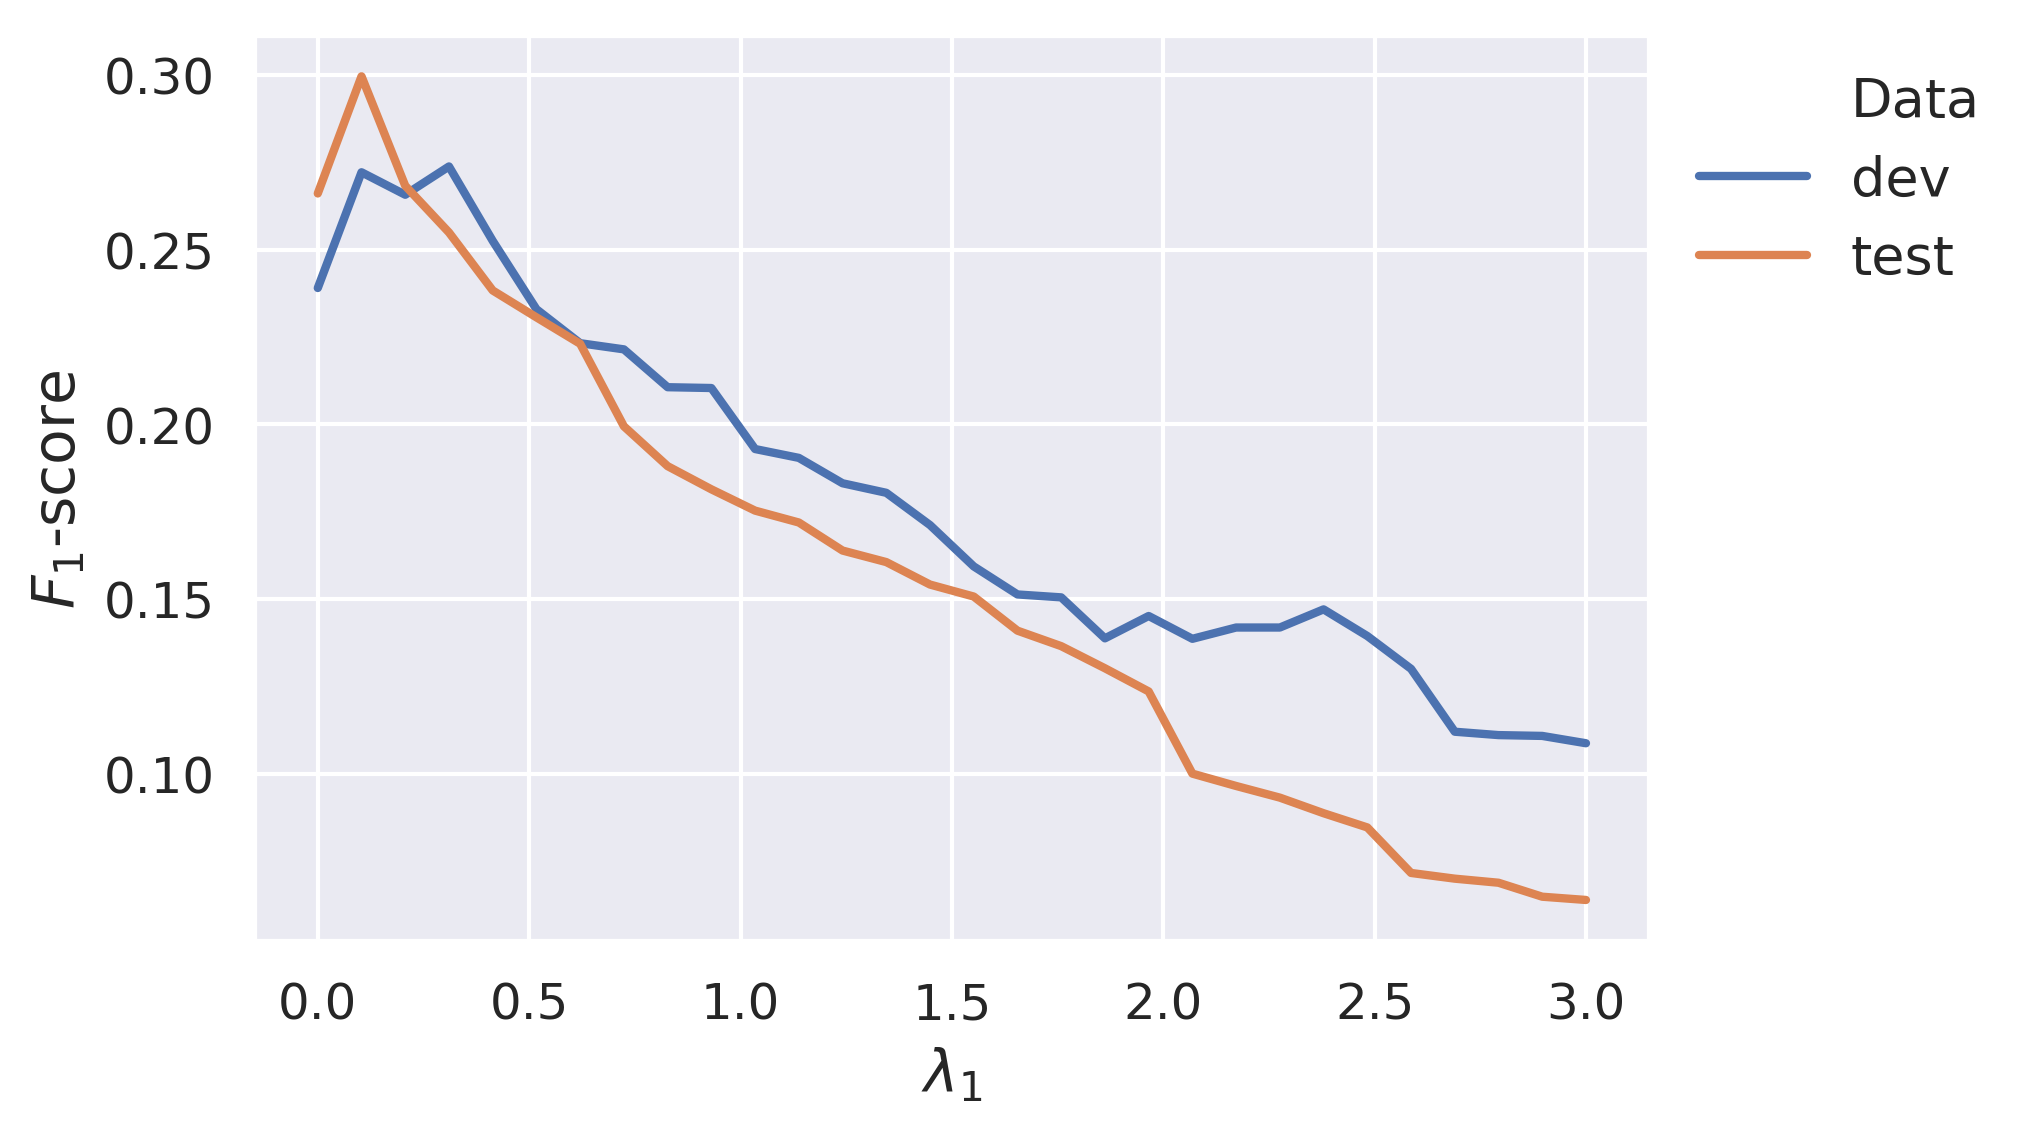
\includegraphics[width=\linewidth]{img/fgsa_lambda1.png}
  \caption{$\lambda_1$}\label{fgsa:fig:crf-lambda1}
\end{subfigure}%
\begin{subfigure}{.5\textwidth}
  \centering
  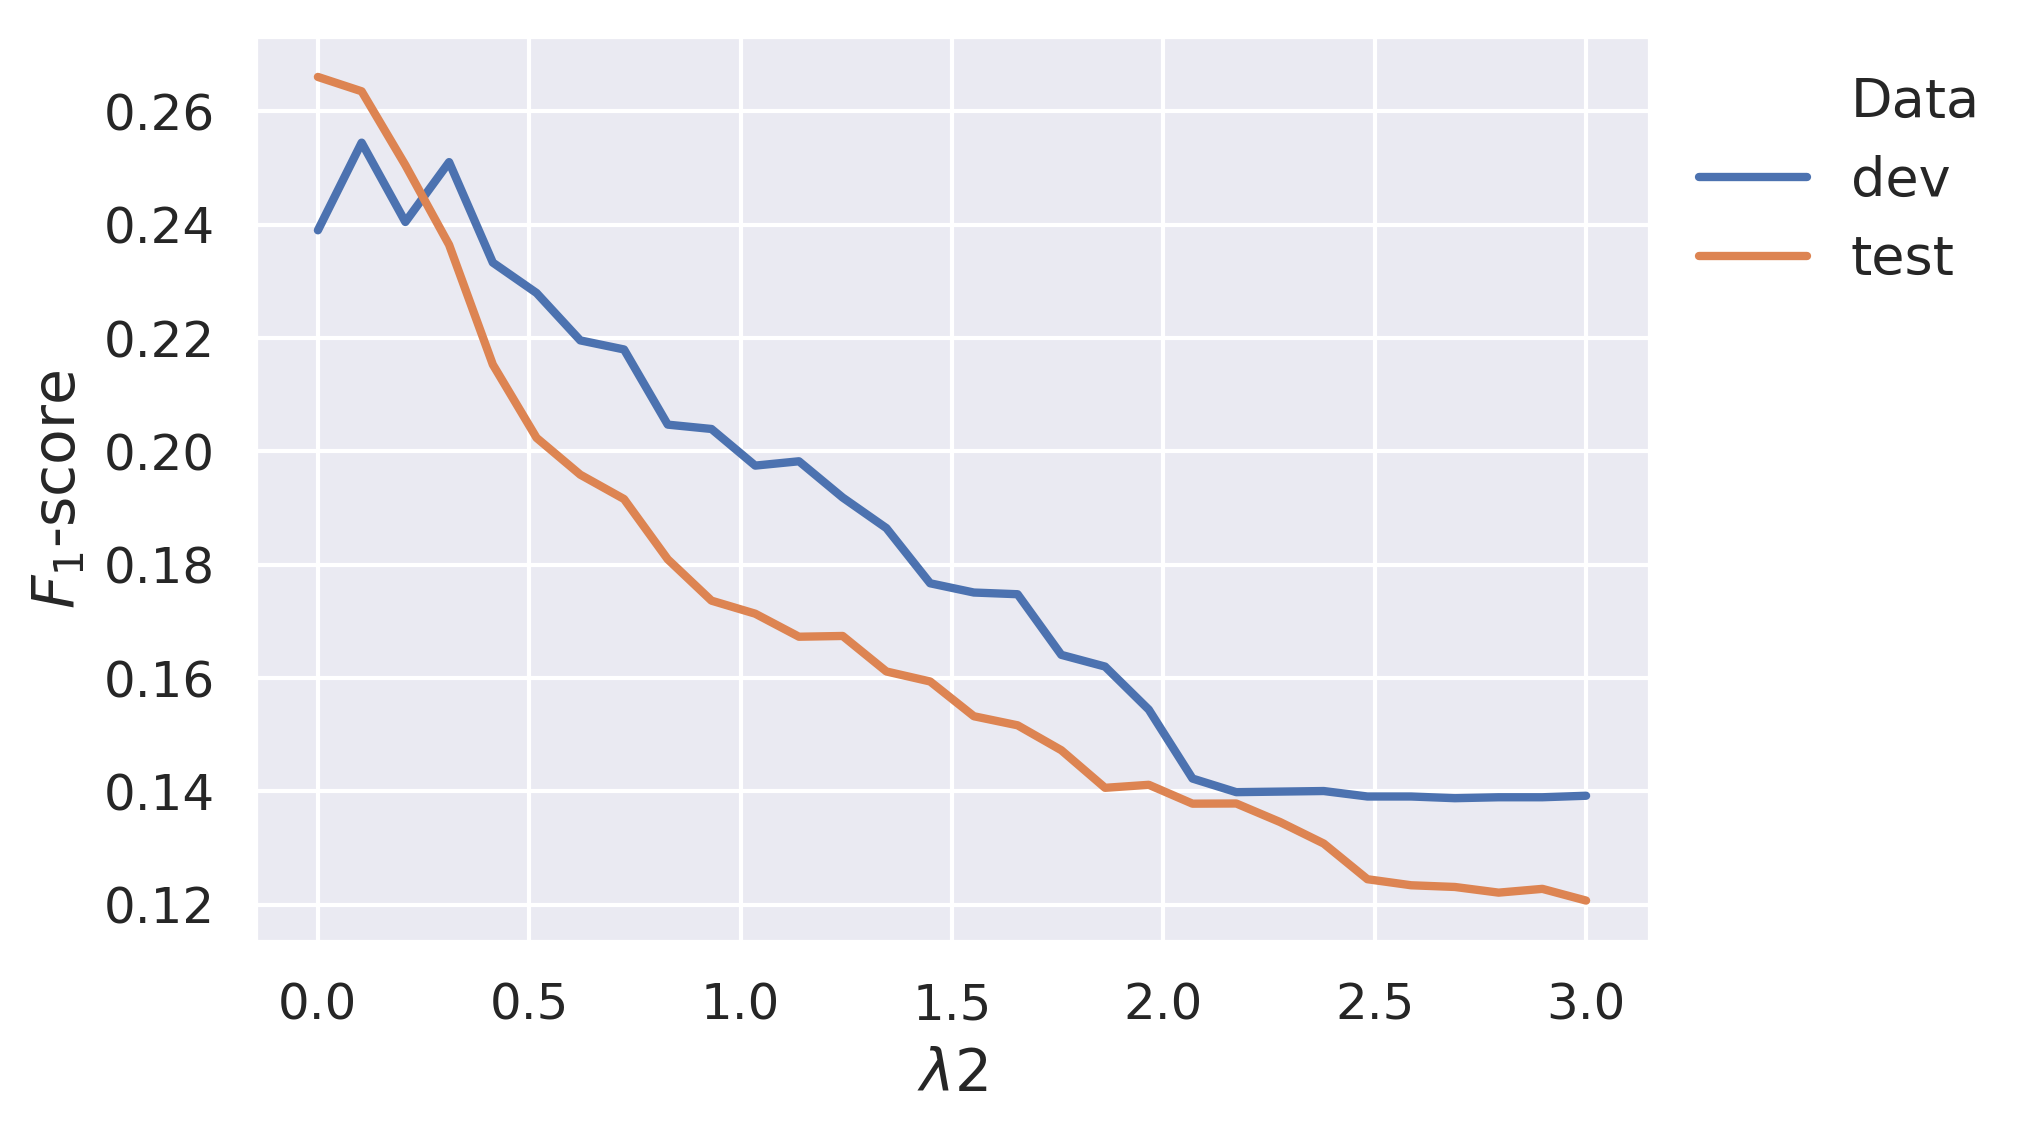
\includegraphics[width=\linewidth]{img/fgsa_lambda2.png}
  \caption{$\lambda_2$}\label{fgsa:fig:crf-lambda2}
\end{subfigure}
}
\caption[CRF results for different regularization values]{Results of
  the linear-chain CRFs with different values of regularization
  parameters}\label{fgsa:fig:crf-regularization}
\end{figure*}

Another factor that could significantly affect the generalization of
the CRF system was the regularization parameters $\lambda_1$ and
$\lambda_2$, which controlled the amount of penalty imposed on too big
learned feature weights (see
Equation~\ref{snt:fgsa:eq:crf-w-regularization}).  Because we chose
these parameters based on the model's results on the held-out
development data, a possible reason for rather low scores on the test
set could be a considerable difference between the distribution of
\markable{sentiment}s, \markable{source}s, and \markable{target}s in
the development and test parts of the corpus.  To see whether it
indeed was the case, we recomputed the \F{}-scores on the development
and test data, using different $\lambda$ values, and present the
results of this computation in
Figure~\ref{fgsa:fig:crf-regularization}.  As is evident from the
figure, model's \F-measure on the development set largely correlates
with its performance on the test corpus, and almost monotonically
decreases with larger $\lambda$s.

\subsection{Error Analysis}

Besides looking into model's parameters, we also decided to analyze
some errors made by the CRF system in order to understand the reasons
for its misclassifications.

\begin{example}[An Error Made by the CRF System]\label{snt:fgsa:exmp:crf-error-1}
%% TARGET  O       TARGET  �berall
%% TARGET  O       TARGET  npd
%% TARGET  O       TARGET  plakat
%% SENTIMENT       O       SENTIMENT       %negsmiley

%% LABELS = {
%%       0: TARGET
%%       1: O
%%       2: SENTIMENT
%%       3: SOURCE
%% }

%% state[0][0] = -2.816934
%% state[0][1] = 6.514906
%% state[0][2] = -3.183343
%% state[0][3] = -3.923175

%% state[1][0] = 7.019282
%% state[1][1] = 5.362580
%% state[1][2] = -0.696150
%% state[1][3] = 1.651658

%% state[2][0] = 3.253026
%% state[2][1] = 0.130018
%% state[2][2] = -1.490348
%% state[2][3] = -5.405246

%% state[3][0] = -5.770071
%% state[3][1] = -1.818361
%% state[3][2] = 2.438365
%% state[3][3] = -9.148613

  \noindent\textup{\bfseries\textcolor{darkred}{Gold Labels:}} {\upshape \"Uberall/TRG NPD/TRG Plakate/TRG \%NegSmiley/SNT}\\
  \noindent Everywhere/TRG NPD/TRG posters/TRG \%NegSmiley/SNT\\[\exampleSep]
  \noindent\textup{\bfseries\textcolor{darkred}{Predicted Labels:}} {\upshape \"Uberall/NON NPD/NON Plakate/NON \%NegSmiley/NON}\\
  \noindent Everywhere/NON NPD/NON posters/NON \%NegSmiley/NON\\[\exampleSep]
\end{example}

One such error is shown in Example~\ref{snt:fgsa:exmp:crf-error-1}.
In this case, the classifier has erroneously overlooked a negative
emoticon, which expresses author's attitude to election posters of the
National Democratic Party of Germany (NPD), and assigned the NON
(none) tags to all tokens of the tweet.  As it turns out, despite this
incorrect assignment, the state potentials of the smiley still achieve
their highest scores with the correct SNT (\markable{sentiment}) tag.
Moreover, the state scores of the word ``Plakate'' (\emph{posters})
also reach their maximum value (0.13 in the logarithmic domain) with
the correct TRG (\markable{target}) label.  Unfortunately, these good
guesses of single tags are overruled by the extremely high score of
the NON label (6.515) that is assigned to the first word of this
message (``\"uberall'' [\emph{everywhere}]) and is reinforced by the
transition features, which prefer contiguous runs of \textsc{NON}s.

This kind of mistakes is by far the most common type of errors that we
have observed on the development set, followed by spans with different
boundaries and invalid label sequences similar to the one shown
Example~\ref{snt:fgsa:exmp:crf-error-2}, where the classifier assigned
only SNT tags to all input tokens, although a \markable{sentiment} in
our original corpus annotation could only appear in the presence of a
\markable{target} element.

\begin{example}[An Error Made by the CRF System]\label{snt:fgsa:exmp:crf-error-2}
%% O	SENTIMENT	O	so
%% O	SENTIMENT	O	m�ssen
%% O	O	O	die
%% O	O	O	sein
%% O	O	O	\%possmiley
%% O	O	O	piraten+

%% LABELS = {
%%       0: TARGET
%%       1: O
%%       2: SENTIMENT
%%       3: SOURCE
%% }

%% state[0][0] = -3.038067
%% state[0][1] = 1.681227
%% state[0][2] = -0.927401
%% state[0][3] = -13.950086

%% state[1][0] = -6.345182
%% state[1][1] = -5.990096
%% state[1][2] = 1.520121
%% state[1][3] = -11.317471

%% state[2][0] = 1.443866
%% state[2][1] = -1.640298
%% state[2][2] = -1.497256
%% state[2][3] = -6.206925

%% state[3][0] = 4.883781
%% state[3][1] = 6.219811
%% state[3][2] = 5.258309
%% state[3][3] = -6.819373

%% state[4][0] = -3.866373
%% state[4][1] = -0.408577
%% state[4][2] = -0.374299
%% state[4][3] = -3.834682

%% state[5][0] = -7.603441
%% state[5][1] = -1.632574
%% state[5][2] = -5.785819
%% state[5][3] = -8.896403

%% SENTIMENT:0.905768
%% SENTIMENT:0.922549
%% O:0.291830
%% O:0.713491
%% O:0.864184
%% O:0.951727
  \noindent\textup{\bfseries\textcolor{darkred}{Gold Labels:}}
                  {\upshape So/SNT muss/SNT das/SNT sein/SNT
                    \%PosSmiley/SNT piraten+/TRG}\\
  \noindent That/SNT 's/SNT the/SNT way/SNT how/SNT it/SNT 's/SNT\\
  supposed/SNT to/SNT be/SNT \%PosSmiley/SNT
  piraten+/TRG\\[\exampleSep]
  \noindent\textup{\bfseries\textcolor{darkred}{Predicted Labels:}}
                  {\upshape So/SNT muss/SNT das/SNT sein/SNT
                    \%PosSmiley/SNT piraten+/SNT}\\
  \noindent That/SNT 's/SNT the/SNT way/SNT how/SNT it/SNT 's/SNT\\
  supposed/SNT to/SNT be/SNT \%PosSmiley/SNT
  piraten+/TRG\\[\exampleSep]
\end{example}

\section{Recurrent Neural Networks}

A competitive alternative to CRFs is deep recurrent neural networks
(RNNs).  Introduced in the mid-nineties~\cite{Hochreiter:97}, RNNs
have become one of the most popular trends in the raging tsunami of
deep learning applications, demonstrating superior results on many
important NLP tasks including part-of-speech
tagging~\cite{Wang:15:pos}, dependency parsing~\cite{Kiperwasser:16a},
and machine
translation~\cite{Kalchbrenner:13,Bahdanau:14,Sutskever:14}.  Key
factors that account for this success are
\begin{enumerate}[1)]
\item \emph{the ability of RNN systems to learn optimal feature
  representations automatically}, which favorably sets them apart from
  traditional supervised machine-learning frameworks, such as SVMs or
  CRFs, where all features need to be defined by the user; and
\item \emph{the ability to deal with arbitrary sequence lengths},
  which advantageously distinguishes these methods from other NN
  architectures, such as plain feed-forward networks or convolutional
  systems without pooling, where the size of the input layer has to be
  constant.
\end{enumerate}

The main component that underlies any modern RNN approach is a
fixed-size hidden vector $\vec{h}$, which is recurrently updated
during the analysis of an input sequence $\mathbf{x}$ and is meant to
encode the meaning of that sequence.  The general form of this vector
at input state $t$ is usually defined as:
\begin{align*}
  \vec{h}^{(t)} = f(\vec{h}^{(t-1)}, \mathbf{x}^{(t)});
\end{align*}
where $f$ represents some non-linear transformation function,
$\vec{h}^{(t-1)}$ denotes the state of the hidden vector at the
previous time step, and $\mathbf{x}^{(t)}$ is the input vector at
position $t$.

\paragraph{LSTM.}

A fundamental problem that arises from the above definition is that
the gradients of model's parameters rapidly vanish to zero or explode
to infinity (depending on whether the absolute values of $\vec{h}$ are
less or greater than one) as the length of the input sequence
increases.  In order to solve this issue, \citet{Hochreiter:97}
proposed the long short-term memory mechanism (LSTM), in which they
explicitly incorporated the goal of keeping the gradients within an
appropriate range.  In particular, given an input sequence
$\mathbf{x}$, they introduced a special \emph{activation unit}
$\vec{i}^{(t)}$:
\begin{align*}
  \vec{i}^{(t)} &= \sigma\left(W_i\cdot \mathbf{x}^{(t)} + U_i \cdot \vec{h}^{(t-1)} + \vec{b}_i\right);
\end{align*}
where $\sigma$ denotes the sigmoid function; $W_i$, $U_i$, and
$\vec{b_i}$ represent model's parameters; $\mathbf{x}^{(t)}$ stands
for the input state; and $\vec{h}^{(t-1)}$ means the previous hidden
state.  In addition to the activation unit, the authors also estimated
a dedicated \emph{forget gate}~$\vec{f}^{(t)}$:
\begin{align*}
  \vec{f}^{(t)} &= \sigma\left(W_f\cdot \mathbf{x}^{(t)} + U_f
  \cdot \vec{h}^{(t-1)} + \vec{b}_f\right),
\end{align*}
which is used to erase parts of the previous input that appear to be
irrelevant.

After computing an \emph{intermediate update state}
$\widetilde{c}^{(t)}$ for the current time step~$t$:
\begin{align*}
  \widetilde{c}^{(t)} &= \tanh\left(W_c\cdot \mathbf{x}^{(t)} + U_c
  \cdot \vec{h}^{(t-1)} + \vec{b}_c\right),
\end{align*}
they estimated the \emph{final update}~$\vec{c}^{(t)}$ by taking a
weighted sum of the candidate update vector~$\widetilde{c}^{(t)}$ and
the previous update value~$\vec{c}^{(t-1)}$:
\begin{align*}
  \vec{c}^{(t)} &= \vec{i}^{(t)} \odot \widetilde{c}^{(t)} +
  \vec{f}^{(t)} \odot \vec{c}^{(t-1)};
\end{align*}
from which, they finally computed the output vector $\vec{o}^{(t)}$
and the new value of the hidden state $\vec{h}^{(t)}$:
\begin{align*}
  \vec{o}^{(t)} &= \sigma\left(W_o\cdot \mathbf{x}^{(t)} + U_o \cdot \vec{h}^{(t-1)} + V_o \cdot \vec{c}^{(t)} + \vec{b}_o\right),\\
  \vec{h}^{(t)} &= \vec{o}^{(t)} \odot \tanh(\vec{c}^{(t)}).
\end{align*}

\paragraph{GRU.}

Despite their enormous
popularity~\cite[\eg{}][]{Filippova:15,Ghosh:16,Rao:16}, LSTMs have
been criticized for the high complexity of their recurrent unit.  In
order to overcome this deficiency, while still keeping the gradients
within an acceptable range, \citet{Cho:14a} proposed an alternative
architecture called Gated Recurrent Units (GRU).  In this framework,
the authors also used activation and forget gates ($\vec{i}^{(t)}$ and
$\vec{f}^{(t)}$) similar to the ones defined by~\citet{Hochreiter:97}:
\begin{align*}
  \vec{i}^{(t)} &= \sigma\left(W_i\cdot \mathbf{x}^{(t)} + U_i \cdot \vec{h}^{(t-1)} + \vec{b}_i\right),\\
  \vec{f}^{(t)} &= \sigma\left(W_f\cdot \mathbf{x}^{(t)} + U_f \cdot \vec{h}^{(t-1)} + \vec{b}_f\right).
\end{align*}
With the help of these gates, they estimated the candidate activation
$\widetilde{c}^{(t)}$ as:
\begin{align*}
  \widetilde{c}^{(t)} &= tanh\left(W_c\cdot \mathbf{x}^{(t)} + U_c
  \cdot \left(\vec{f}^{(t)} \odot \vec{h}^{(t-1)}\right)  + \vec{b}_c\right),
\end{align*}
and computed the hidden state $\vec{h}^{(t)}$ as:
\begin{align*}
  \vec{h}^{(t)} &= \vec{i}^{(t)} \odot \vec{h}^{(t-1)} + \left(\vec{1} -
  \vec{i}^{(t)}\right) \odot \widetilde{c}^{(t)}.
\end{align*}

\paragraph{Final Layer.}

Because the output vectors of these recurrences ($\vec{o}^{(t)}$ in
the LSTM case, and $\vec{h}^{(t)}$ in the case of GRU) do not strictly
represent label probabilities (since elements of these vectors can
also be negative and typically do not sum to one), and, moreover,
because the size of our tagset (four tags: \textsc{SNT}, \textsc{SRC},
\textsc{TRG}, and \textsc{NON}) was obviously too small for the size
of the hidden unit, we set the dimensionality of the intermediate RNN
vectors to 100, and apply a linear transformation matrix $O \in
\mathbb{R}^{4 \times 100}$ to the final output of the recursion loop,
computing the softmax of their dot product:
\begin{align*}
  \vec{p}^{(t)} &= softmax\left(O\cdot\vec{o}^{(t)}\right).
\end{align*}
and considering the greatest value in the resulting vector as the
probability of the most likely tag.

\paragraph{Training.}

A neat property of LSTM and GRU is that the final equation, which is
obtained after unrolling the recurrence loop, is differentiable with
respect to all of its parameters, and can therefore be optimized with
standard gradient update techniques.  Since most of these parameters,
however, represent high-dimensional matrices or vectors, finding an
optimal learning rate (\ie{} the size of the update step taken in the
direction of the gradient) might pose considerable difficulties,
leading either to prohibitively large training times (if the steps are
too small) or complete divergence of the trained model (if the steps
are too large).

Several algorithms have been proposed for solving this problem,
including the method of momentum~\cite{Rumelhart:88},
AdaGrad~\cite{Duchi:11}, AdaDelta~\cite{Zeiler:12},
RMSProp~\cite{Tieleman:12}, etc.  In our experiments, we used the last
of these options---RMSProp~\cite{Tieleman:12}---as this algorithm
showed both a faster convergence and better classification results.

Another important factor that could significantly influence the
results were initial values of models' parameters.  As shown
by~\citet{He:15}, an inappropriate initialization of neural network
might lead to a complete stalling of the whole learning process.
Following recommended practices~\cite{Saxe:13}, we used orthogonal
initialization for all linear transformation matrices, and applied
uniform He sampling~\cite{He:15} for setting the initial values of
bias vectors.

Finally, due to a high imbalance of the target classes in the training
set (where most of the instances represent objective statements
without any sentiment tags), we ``upsampled'' sentiment tweets (\ie{}
we randomly repeated microblogs containing \markable{sentiment}s until
we reached an equal proportion of subjective and objective messages),
and chose the \emph{hinge-loss} as the optimized objective function
$L$:\footnote{Since most of the tokens in the over-sampled training
  set still have the \textsc{NON} tag, the easiest way for a
  classifier to minimize the objective function is to always predict
  this tag with a very high confidence.  We hoped to mitigate this
  effect by using the hinge-loss, since this function only penalizes
  incorrectly predicted labels or correct tags whose probability is
  insufficiently high (less than $c$), but does not reward any
  over-confident decisions.}
\begin{align}
  L &= \sum_{i}^{N}\sum_{t=0}^{\lvert\mathbf{x}_i\rvert}\max\left(0, %
  c + \max\limits_{y'\neq y}\vec{p}_{t,y'} - \vec{p}_{t,y}\right) + \alpha \norm{O}^2_2,
\end{align}
where $\vec{p}_{t,y'}$ stands for the probability of the most likely
wrong tag $y'$ at position $t$ in the training instance
$\mathbf{x}_i$, $\vec{p}_{t,y}$ represents the probability of the gold
label, and $\norm{O}^2_2$ stands for the $L2$-norm of the $O$ matrix.

We optimized the scalar hyper-parameters $c$ and $\alpha$ on the
development set, and trained the final model for 256 epochs, choosing
parameter values that maximized the macro-averaged \F-score on the
development set.

\paragraph{Inference.}

Since each of the above approaches (LSTM and GRU) explicitly defines
an output unit, the inference of the most likely label assignment for
an input instance $\mathbf{x}$ is straightforward and amounts to
finding the $\argmax$ value of the output vector at each time step of
the recurrence:
\begin{equation*}
  \mathbf{\hat{y}} =
  \argmax{\vec{p}^{(1)}},\argmax{\vec{p}^{(2)}},\ldots,\argmax{\vec{p}^{(|\mathbf{x}|)}}.
\end{equation*}

\paragraph{Results.}

To account for the random factors in the initialization, we repeated
each training experiment three times, and show the mean and the
standard deviation of these results in
Table~\ref{snt-fgsa:tbl:rnn-res}.

As we can see from the table, the LSTM model shows generally better
scores than the GRU system on both training and test sets.  The only
aspect at which it yields slightly worse results than the latter
approach is precision of \markable{sentiment}s, which, however, is
more than compensated for by a much higher recall.  Moreover, the
overfitting effect is significantly less pronounced than in the CRF
case (where the \F{}-scores on the training and test data differed by
a factor of three).  Nonetheless, both RNN systems achieve lower
results than the linear-chain CRFs, which indicates the fact that the
learned features still cannot capture the full extent of information
that a human expert can encode with manually defined attributes.

\begin{table*}
  \begin{center}
    \bgroup \setlength\tabcolsep{0.1\tabcolsep}\scriptsize
    \begin{tabular}{p{0.162\columnwidth} % first columm
        *{9}{>{\centering\arraybackslash}p{0.074\columnwidth}} % next nine columns
        *{1}{>{\centering\arraybackslash}p{0.136\columnwidth}}} % last two columns
      \toprule
      \multirow{2}*{\bfseries Data Set} & \multicolumn{3}{c}{\bfseries Sentiment} & %
      \multicolumn{3}{c}{\bfseries Source} & %
      \multicolumn{3}{c}{\bfseries Target} & %
      \multirow{2}{0.136\columnwidth}{\bfseries\centering Macro\newline \F{}}\\\cmidrule(lr){2-4}\cmidrule(lr){5-7}\cmidrule(lr){8-10}
      & Precision & Recall & \F{} & %
      Precision & Recall & \F{} & %
      Precision & Recall & \F{} &\\\midrule

      \multicolumn{11}{c}{\cellcolor{cellcolor}LSTM}\\
      %%  Tag        Precision    Recall F-Measure
      %% O             86.60%    86.63%    86.62%
      %% SENTIMENT     55.50%    74.72%    63.69%
      %% SOURCE        46.27%    68.82%    55.33%
      %% TARGET        43.12%    77.99%    55.53%

      %% Tag        Precision    Recall F-Measure
      %% O             88.76%    67.71%    76.82%
      %% SENTIMENT     30.76%    76.51%    43.88%
      %% SOURCE        38.84%    49.82%    43.65%
      %% TARGET        29.45%    67.18%    40.95%

      %% Tag        Precision    Recall F-Measure
      %% O             86.38%    89.91%    88.11%
      %% SENTIMENT     60.90%    74.87%    67.16%
      %% SOURCE        48.96%    71.18%    58.02%
      %% TARGET        50.61%    74.58%    60.30%

      Training Set & 0.49\stddev{0.16} & 0.75\stddev{0.01} & 0.58\stddev{0.13} & %
      0.45\stddev{0.05} & 0.63\stddev{0.12} & 0.52\stddev{0.08} %
      & 0.41\stddev{0.11} & 0.73\stddev{0.06} & 0.52\stddev{0.11} %
      & 0.54\stddev{0.11}\\

      %% Tag        Precision    Recall F-Measure
      %% O             77.77%    82.91%    80.26%
      %% SENTIMENT     31.69%    28.00%    29.73%
      %% SOURCE        23.05%    31.25%    26.53%
      %% TARGET        21.77%    23.57%    22.63%

      %% Tag        Precision    Recall F-Measure
      %% O             79.83%    71.62%    75.50%
      %% SENTIMENT     26.23%    43.07%    32.60%
      %% SOURCE        26.07%    30.68%    28.19%
      %% TARGET        21.53%    30.16%    25.13%

      %% Tag        Precision    Recall F-Measure
      %% O             77.58%    86.08%    81.61%
      %% SENTIMENT     30.16%    22.60%    25.84%
      %% SOURCE        24.42%    30.60%    27.16%
      %% TARGET        24.99%    21.20%    22.94%

      Test Set & 0.29\stddev{0.03} & \textbf{0.31}\stddev{0.11} & \textbf{0.29}\stddev{0.03} &%
      \textbf{0.25}\stddev{0.02} & \textbf{0.31}\stddev{0.0} & \textbf{0.27}\stddev{0.01} & %
      \textbf{0.23}\stddev{0.02} & \textbf{0.25}\stddev{0.05} & \textbf{0.24}\stddev{0.01} & %
      \textbf{0.27}\stddev{0.02}\\

      \multicolumn{11}{c}{\cellcolor{cellcolor}GRU}\\

      %% Tag        Precision    Recall F-Measure
      %% O             82.40%    89.44%    85.77%
      %% SENTIMENT     60.16%    60.25%    60.21%
      %% SOURCE        44.77%    66.74%    53.59%
      %% TARGET        46.36%    63.22%    53.49%

      %% Tag        Precision    Recall F-Measure
      %% O             87.39%    80.32%    83.71%
      %% SENTIMENT     44.88%    70.75%    54.92%
      %% SOURCE        39.69%    63.31%    48.79%
      %% TARGET        35.37%    73.96%    47.86%

      %% Tag        Precision    Recall F-Measure
      %% O             81.03%    87.80%    84.28%
      %% SENTIMENT     47.95%    66.84%    55.84%
      %% SOURCE        42.49%    56.86%    48.64%
      %% TARGET        58.22%    51.08%    54.42%

      Training Set & 0.51\stddev{0.08} & 0.66\stddev{0.05} & 0.57\stddev{0.03} & %
      0.42\stddev{0.03} & 0.62\stddev{0.05} & 0.5\stddev{0.03} & %
      0.47\stddev{0.11} & 0.63\stddev{0.11} & 0.52\stddev{0.04} & 0.53\stddev{0.03}\\

      %% Tag        Precision    Recall F-Measure
      %% O             76.78%    86.47%    81.34%
      %% SENTIMENT     30.77%    19.68%    24.01%
      %% SOURCE        20.71%    26.44%    23.22%
      %% TARGET        24.20%    20.93%    22.45%

      %% Tag        Precision    Recall F-Measure
      %% O             78.15%    79.14%    78.64%
      %% SENTIMENT     28.61%    30.25%    29.41%
      %% SOURCE        19.71%    29.45%    23.62%
      %% TARGET        21.54%    27.49%    24.15%

      %% Tag        Precision    Recall F-Measure
      %% O             77.52%    86.03%    81.56%
      %% SENTIMENT     30.66%    28.43%    29.50%
      %% SOURCE        24.46%    29.09%    26.58%
      %% TARGET        27.17%    14.15%    18.61%

      Test Set & \textbf{0.3}\stddev{0.01} & 0.26\stddev{0.06} & 0.28\stddev{0.03} & %
      0.22\stddev{0.03} & 0.28\stddev{0.02} & 0.24\stddev{0.02} & %
      0.24\stddev{0.03} & 0.21\stddev{0.07} & 0.22\stddev{0.03} & 0.25\stddev{0.01}\\\bottomrule
    \end{tabular}
    \egroup
    \caption{Results of fine-grained sentiment analysis with recurrent
      neural networks}
    \label{snt-fgsa:tbl:rnn-res}
  \end{center}
\end{table*}

\subsection{Word Embeddings}

To see whether using different embeddings would improve the results of
the tested methods, we reran our experiments with two alternative
embedding types:
\begin{itemize}
\item \emph{word2vec vectors}~\cite{Mikolov:13}, which had been
  pretrained on the German Twitter snapshot~\cite{Scheffler:14} and
  were kept fixed during the RNN optimization;
\item and \emph{least-squares embeddings}, which were previously
  described in Chapter~\ref{chap:snt:lex};
\end{itemize}
subsequently evaluating all systems on the development set.

The results of this evaluation are shown in
Table~\ref{snt-fgsa:tbl:embeddings}.  As we can see from the scores,
least-squares representations significantly improve the recall of all
classes, which, in turn, leads to much higher macro-averaged
\F-measures in comparison with other embeddings.  The task-specific
variant shows second-best results, mainly due to a higher precision of
\markable{target}s and \markable{source}s.  Finally, word2vec vectors
also improve the prediction of \markable{sentiment} spans, but
otherwise cause a notable degradation of literally every other aspect.

\begin{table*}
  \begin{center}
    \bgroup \setlength\tabcolsep{0.1\tabcolsep}\scriptsize
    \begin{tabular}{p{0.162\columnwidth} % first columm
        *{9}{>{\centering\arraybackslash}p{0.074\columnwidth}} % next nine columns
        *{1}{>{\centering\arraybackslash}p{0.136\columnwidth}}} % last two columns
      \toprule
      \multirow{2}*{\bfseries RNN} & \multicolumn{3}{c}{\bfseries Sentiment} & %
      \multicolumn{3}{c}{\bfseries Source} & %
      \multicolumn{3}{c}{\bfseries Target} & %
      \multirow{2}{0.136\columnwidth}{\bfseries\centering Macro\newline \F{}}\\\cmidrule(lr){2-4}\cmidrule(lr){5-7}\cmidrule(lr){8-10}
      & Precision & Recall & \F{} & %
      Precision & Recall & \F{} & %
      Precision & Recall & \F{} &\\\midrule

      \multicolumn{11}{c}{\cellcolor{cellcolor}Task-Specific Embeddings}\\

      LSTM & 0.283 & 0.288 & 0.278 & %
       \textbf{0.293} & 0.372 & 0.328 & %
       \textbf{0.254} & 0.27 & \textbf{0.259} & 0.288\\

      GRU & 0.287 & 0.246 & 0.263 & %
       0.287 & 0.405 & \textbf{0.335} & %
       0.252 & 0.205 & 0.216 & 0.271\\

      \multicolumn{11}{c}{\cellcolor{cellcolor}Least-Squares Embeddings}\\

      LSTM & 0.268 & \textbf{0.37} & 0.307 & %
      0.261 & \textbf{0.414} & 0.314 & %
      0.223 & \textbf{0.275} & 0.245 & \textbf{0.289}\\

      GRU & 0.256 & 0.341 & 0.291 & %
       0.267 & 0.395 & 0.318 & %
       0.229 & 0.262 & 0.245 & 0.285\\

      \multicolumn{11}{c}{\cellcolor{cellcolor}word2vec Embeddings}\\

      LSTM & \textbf{0.291} & 0.329 & \textbf{0.309} & %
       0.2 & 0.311 & 0.244 & %
       0.221 & 0.219 & 0.22 & 0.257\\

      GRU & 0.273 & 0.355 & 0.301 & %
       0.207 & 0.353 & 0.257 & %
       0.213 & 0.26 & 0.233 & 0.264\\\bottomrule
    \end{tabular}
    \egroup
    \caption{Results of fine-grained sentiment analysis with different
      word embeddings}
    \label{snt-fgsa:tbl:embeddings}
  \end{center}
\end{table*}

\subsection{Error Analysis}

As in the previous case, we also decided to have a closer look at some
sample errors, which were committed by the tested systems.  As it
turned out, the most common type of mistakes made by both classifiers
was confusion of NON labels with other tags, which we also can see in
Examples~\ref{snt:fgsa:exmp:lstm-error} and
\ref{snt:fgsa:exmp:gru-error}.

\begin{example}[An Error Made by the LSTM System]\label{snt:fgsa:exmp:lstm-error}
  \noindent\textup{\bfseries\textcolor{darkred}{Gold Labels:}}
                  {\upshape Meine/NON Mama/NON liest/NON bei/NON
                    Twitter/NON mit/NON}\\
  \noindent My/NON mom/NON is/NON reading/NON Twitter/NON together/NON
  with/NON me/NON\\[\exampleSep]
  \noindent\textup{\bfseries\textcolor{darkred}{Predicted Labels:}}
                  {\upshape Meine/TRG Mama/NON liest/NON bei/NON
                    Twitter/NON mit/NON}\\
  \noindent My/TRG mom/NON is/NON reading/NON Twitter/NON together/NON
  with/NON me/NON\\[\exampleSep]
\end{example}

The obvious reason for these wrong predictions was the upsampling of
sentiment tweets that we used to balance the class distribution in the
training data.  Unfortunately, switching this component off caused all
classifiers to always predict only the NON tag and significantly
worsened the scores of these approaches in comparison with our initial
experiments.

\begin{example}[An Error Made by the GRU System]\label{snt:fgsa:exmp:gru-error}
  \noindent\textup{\bfseries\textcolor{darkred}{Gold Labels:}}
                  {\upshape Ich/NON habe/NON das/NON ``noch''/NON\\
                    vergessen/NON}\\
  \noindent I/NON have/NON forgotten/NON the/NON ``still''/NON\\[\exampleSep]
  \noindent\textup{\bfseries\textcolor{darkred}{Predicted Labels:}}
                  {\upshape Ich/SRC habe/NON das/TRG ``noch''/NON\\
                    vergessen/NON}\\
  \noindent I/SRC have/NON forgotten/NON the/TRG ``still''/NON\\[\exampleSep]
\end{example}

\section{Evaluation}

After estimating the results of popular FGSA approaches with their
(mostly) standard settings, evaluating their specific components
(features and word embeddings), and looking at their sample errors, we
also decided to investigate the impact of common factors, such as
annotation scheme, graph structure, and text normalization on the net
results of these methods.  For this purpose, we reran the evaluation,
changing one aspect of the training procedure at a time, and
re-estimated the scores of these systems on the development set.  The
results of these experiments are presented below.

\subsection{Annotation Scheme}

As the first factor that could affect the quality of automatic FGSA
methods, we considered the annotation scheme that we used to create
the corpus.  As described in Section~\ref{subsec:snt:ascheme}, we
initially asked our experts to assign the \markable{sentiment} label
to complete syntactic or discourse-level units that included both the
target of an opinion and its immediate evaluative expression.  Even
though this decision was linguistically plausible and helpful for
determining the boundaries of \markable{sentiment}s and their relevant
components, it also posed considerable difficulties for sequence
labeling techniques, since \markable{sentiment} tags were assigned not
only to the immediate polar terms but also to neutral words that
occurred within the same syntactic constituent as the polar item and
its target.  Since none of the tested methods could explicitly
incorporate this logic, we decided to check whether an alternative
interpretation of the annotation scheme could alleviate their
inference.

In particular, instead of unconditionally labeling all words belonging
to a \markable{sentiment} span in the original annotation with the
\textsc{SNT} tag as we did previously (which we call a \emph{broad}
interpretation of the annotation scheme), we only assigned this label
to the polar terms found in the corpus (which we call a \emph{narrow}
interpretation).  The difference between these two takes is shown in
Examples~\ref{snt:fgsa:exmp:wide} and~\ref{snt:fgsa:exmp:narrow}.
\begin{example}[Broad Sentiment
  Interpretation]\label{snt:fgsa:exmp:wide}
  \noindent\sentiment{\target{Francis} makes a \intensifier{very}
    \emoexpression{good} impression on\\ \source{me}!
    \emoexpression{:)}}

  $\rightarrow$

  \noindent Francis/TRG makes/SNT a/SNT very/SNT good/SNT
  impression/SNT on/SNT\\ me/SRC !/SNT :)/SNT
\end{example}

\begin{example}[Narrow Sentiment Interpretation]\label{snt:fgsa:exmp:narrow}
  \noindent\sentiment{\target{Francis} makes a \intensifier{very}
    \emoexpression{good} impression on\\ \source{me}!
    \emoexpression{:)}}

  $\rightarrow$

  \noindent Francis/TRG makes/NON a/NON very/NON good/SNT
  impression/NON on/NON\\ me/SRC !/NON :)/SNT
\end{example}
\noindent In the former (broad) case, we labeled the whole subjective
sentence with the \textsc{SNT} tag except for the words that denoted
the target and source of the opinion.  In the latter (narrow) case, we
only assigned the \textsc{SNT} tag to the polar term ``good'' and the
emoticon ``:),'' which, however, were expressive enough to convey the
main evaluative sense of the whole subjective statement.

\begin{table*}[hbt!]
  \begin{center}
    \bgroup \setlength\tabcolsep{0.1\tabcolsep}\scriptsize
    \begin{tabular}{p{0.162\columnwidth} % first columm
        *{9}{>{\centering\arraybackslash}p{0.074\columnwidth}} % next nine columns
        *{1}{>{\centering\arraybackslash}p{0.136\columnwidth}}} % last two columns
      \toprule
      \multirow{2}*{\bfseries Method} & \multicolumn{3}{c}{\bfseries Sentiment} & %
      \multicolumn{3}{c}{\bfseries Source} & %
      \multicolumn{3}{c}{\bfseries Target} & %
      \multirow{2}{0.136\columnwidth}{\bfseries\centering Macro\newline \F{}}\\\cmidrule(lr){2-4}\cmidrule(lr){5-7}\cmidrule(lr){8-10}
      & Precision & Recall & \F{} & %
      Precision & Recall & \F{} & %
      Precision & Recall & \F{} &\\\midrule

      \multicolumn{11}{c}{\cellcolor{cellcolor}Broad Interpretation}\\

      %% SENTIMENT     37.62%    31.85%    34.49%
      %% SOURCE        29.75%    33.00%    31.29%
      %% TARGET        29.25%    23.06%    25.79%

      CRF & 0.38 & 0.32 & 0.34 & %
      \textbf{0.3} & 0.33 & 0.31 & %
      \textbf{0.29} & 0.23 & \textbf{0.26} & 0.31\\

      % Tag        Precision    Recall F-Measure
      % O             77.89%    70.02%    73.75%
      % SENTIMENT     24.03%    37.51%    29.29%
      % SOURCE        28.52%    37.43%    32.37%
      % TARGET        22.73%    30.54%    26.06%

      % Tag        Precision    Recall F-Measure
      % O             76.44%    86.10%    80.98%
      % SENTIMENT     30.53%    23.22%    26.38%
      % SOURCE        27.74%    36.33%    31.46%
      % TARGET        28.76%    23.59%    25.92%

      % Tag        Precision    Recall F-Measure
      % O             76.87%    83.75%    80.16%
      % SENTIMENT     30.39%    25.69%    27.84%
      % SOURCE        31.59%    37.88%    34.45%
      % TARGET        24.59%    26.94%    25.71%

      % Summary:
      % Tag             Precision    Recall        F1
      % SENTIMENT           28.32     28.81     27.84
      % SOURCE              29.28     37.21     32.76
      % TARGET              25.36     27.02     25.90
      % Macro-F1  28.8311

      LSTM & 0.28 & 0.29 & 0.28 & %
      0.29 & \textbf{0.37} & \textbf{0.33} & %
      0.25 & \textbf{0.27} & \textbf{0.26} & 0.29\\

      % Tag        Precision    Recall F-Measure
      % O             76.64%    86.78%    81.39%
      % SENTIMENT     30.31%    19.73%    23.90%
      % SOURCE        27.54%    39.00%    32.28%
      % TARGET        23.10%    19.12%    20.93%

      % Tag        Precision    Recall F-Measure
      % O             77.05%    78.92%    77.97%
      % SENTIMENT     28.27%    28.35%    28.31%
      % SOURCE        27.30%    43.05%    33.41%
      % TARGET        22.68%    29.29%    25.56%

      % Tag        Precision    Recall F-Measure
      % O             76.82%    85.63%    80.98%
      % SENTIMENT     27.49%    25.78%    26.60%
      % SOURCE        31.34%    39.30%    34.87%
      % TARGET        29.86%    13.15%    18.26%

      % Summary
      % Tag             Precision    Recall        F1
      % SOURCE              28.73     40.45     33.52
      % SENTIMENT           28.69     24.62     26.27
      % TARGET              25.21     20.52     21.58
      % Macro-F1  27.1244

      GRU & 0.29 & 0.25 & 0.26 & %
       0.29 & 0.4 & 0.34 & %
       0.25 & 0.21 & 0.22 & 0.27\\

      \multicolumn{11}{c}{\cellcolor{cellcolor}Narrow Interpretation}\\

      %% Tag        Precision    Recall F-Measure
      %% O             85.93%    85.69%    85.81%
      %% SENTIMENT     58.84%    64.49%    61.54%
      %% SOURCE        26.13%    23.00%    24.47%
      %% TARGET        22.14%    20.14%    21.09%

      CRF & 0.59 & 0.64 & 0.62 & %
      0.26 & 0.23 & 0.24 & %
      0.22 & 0.20 & 0.21 & 0.36\\

      % Tag        Precision    Recall F-Measure
      % O             85.08%    90.61%    87.76%
      % SENTIMENT     57.18%    66.52%    61.50%
      % SOURCE        27.22%    40.25%    32.48%
      % TARGET        25.54%    12.56%    16.84%

      % Tag        Precision    Recall F-Measure
      % O             84.57%    91.93%    88.10%
      % SENTIMENT     69.83%    60.92%    65.07%
      % SOURCE        32.28%    35.55%    33.84%
      % TARGET        26.04%    16.18%    19.96%

      % Tag        Precision    Recall F-Measure
      % O             84.05%    91.82%    87.77%
      % SENTIMENT     58.79%    67.52%    62.85%
      % SOURCE        30.90%    27.85%    29.30%
      % TARGET        27.07%    13.31%    17.85%

      LSTM & \textbf{0.62} & \textbf{0.65} & \textbf{0.63} & %
      \textbf{0.3} & 0.35 & 0.32 & %
      0.26 & 0.14 & 0.18 & \textbf{0.38}\\

      %% Tag        Precision    Recall F-Measure
      %% O             84.78%    87.61%    86.17%
      %% SENTIMENT     59.02%    61.71%    60.34%
      %% SOURCE        27.35%    37.83%    31.75%
      %% TARGET        22.37%    21.18%    21.76%

      %% Tag        Precision    Recall F-Measure
      %% O             84.38%    90.46%    87.31%
      %% SENTIMENT     60.14%    64.76%    62.36%
      %% SOURCE        27.93%    29.53%    28.71%
      %% TARGET        27.40%    20.07%    23.17%

      % Tag        Precision    Recall F-Measure
      % O             84.98%    85.60%    85.29%
      % SENTIMENT     65.71%    61.64%    63.61%
      % SOURCE        29.91%    31.20%    30.54%
      % TARGET        19.18%    31.63%    23.88%

      GRU & \textbf{0.62} & 0.63 & 0.62 & %
      0.28 & 0.33 & 0.3 & %
      0.23 & 0.24 & 0.23 & \textbf{0.38}\\\bottomrule

    \end{tabular}
    \egroup
    \caption{Results of fine-grained analysis with broad and narrow
      sentiment interpretations}
    \label{snt-fgsa:tbl:broad-narrow}
  \end{center}
\end{table*}

The results of the automatic systems with these two approaches are
given in Table~\ref{snt-fgsa:tbl:broad-narrow}.  As we can see from
the table, the broad interpretation generally leads to notably lower
scores for \markable{sentiment} spans, but yields much better results
for their \markable{source}s and \markable{target}s.  An opposite
situation is observed with the narrow scheme: even though the
\F-values for \markable{sentiment}s are twice as high as in the broad
case, the scores for the remaining elements are up to seven percent
lower.

An obvious explanation for these results is the expected better
amenability of the narrow scheme to the prediction of
\markable{sentiment} labels: since \markable{sentiment} tags are only
assigned to obvious polar terms, it becomes easier for the models to
infer this class using their state features, especially morphological
or lexical ones, or word embeddings.  But, on the other hand, such
short spans lead to disrupted label chains for other opinion-related
elements, setting \markable{sentiment} tags far apart from the spans
of their respective \markable{source}s and \markable{target}s.  As a
consequence, these classes suffer from the lack of context and become
heavily dependent on the state attributes as well.  But, this time,
the effect of state features is rather negative, because in contrast
to \markable{polar term}s, being a source or a target of an opinion is
not an inherent property of the lexical term, but arises solely from
the context which this term appears in.

Consider, for instance, the name ``Silvio Berlusconi'' in
Example~\ref{snt:fgsa:trg-ctxt}, where it appears as the target of a
sentiment in the first sentence (which expresses author's hope that
Silvio Berlusconi will not be the new Pope), but serves as a normal
subject of an objective clause in the second case.  The decision about
the role of this name depends primarily on the sense of the whole
statement rather than the name itself.  Consequently, state attributes
might only increase our prior belief that certain words would rather
appear in a subjective context, but cannot tell for sure whether they
actually do so or not.\footnote{The negative effect of state features
  on prediction of \markable{source}s and \markable{target}s was
  actually observed in our corpus, where one of the most frequently
  made mistakes was the unconditional assignment of the TRG tag to the
  word ``Nordkorea'' (\emph{North Korea}) regardless of its
  surrounding context.}  As a consequence, prediction of
\markable{source}s and \markable{target}s becomes much harder when
they do not have enough context information.

\begin{example}[Contextual Dependence of Target
  Elements]\label{snt:fgsa:trg-ctxt}
  Hoffentlich ist es nicht \target{Silvio Berlusconi}. \#Papst\\[0.5em]
  \noindent Hopefully, this won't be \target{Silvio Berlusconi}. \#Pope\\[1em]
  Silvio Berlusconi ist ein italienischer Medienmagnat und Politiker.\\[0.5em]
  \noindent Silvio Berlusconi is an Italian media tycoon and politician.\\
\end{example}

\subsection{Graph Structure}

Since the lack of contextual links played an important role for
prediction of \markable{source}s and \markable{target}s, we decided to
investigate whether redefining the way these links were established in
the models would improve the results.  For this purpose, we
implemented three possible extensions to the traditional first-order
linear-chain CRFs, which are shown in Figure~\ref{fig:snt:ho-crf}:
\begin{itemize}
  \item higher-order linear-chain CRFs,
  \item first- and higher-order semi-Markov models, and
  \item tree-structured CRFs.\footnote{The training and inference
    algorithms of these CRF variants are described in
    Appendix~\ref{chap:apdx:crf-inference}.}
\end{itemize}

\begin{figure*}[thb]
  \centering
  \begin{subfigure}[t]{0.4\textwidth}
    \centering
      {\scriptsize
  \begin{tikzpicture}
    \tikzstyle{xnode}=[circle,draw,fill=gray76,minimum size=2.3em] %
    \tikzstyle{ynode}=[circle,draw,inner sep=1pt] %
    \tikzstyle{factor}=[rectangle,fill=black,midway,inner sep=0pt,%
    minimum size=0.4em] %
    \tikzstyle{ctxt}=[red] %

    \node[ynode] (SNT1) at (2, 2) {SNT};

    \node[ynode] (TRG1) [above=0.4em of SNT1] {TRG};
    \node[ynode] (SRC1) [above=0.4em of TRG1] {SRC};
    \node[ynode] (NON1) [above=0.4em of SRC1] {NON};

    \node[ynode] (SNT0) [left=2.5em of SNT1] {SNT};

    \node[ynode] (TRG0) [above=0.4em of SNT0] {TRG};
    \node[ynode] (SRC0) [above=0.4em of TRG0] {SRC};
    \node[ynode] (NON0) [above=0.4em of SRC0] {NON};

    \node[xnode] (FEAT1) [below left=2em and 1.7em of SNT1] {};
    \node[xnode] (FEAT2) [below=1.2em of SNT1] {};
    \node[xnode] (FEAT3) [below right=2em and 1.7em of SNT1] {};

    \path [-] (FEAT1) edge node [factor] {} (SNT1);
    \path [-] (FEAT2) edge node [factor] {} (SNT1);
    \path [-] (FEAT3) edge node [factor] {} (SNT1);

    \path [-] (SNT0) edge[ctxt] node [factor,ctxt] {} (SNT1);
    \path [-] (TRG0) edge[ctxt] node [factor,ctxt] {} (SNT1);
    \path [-] (SRC0) edge[ctxt] node [factor,ctxt] {} (SNT1);
    \path [-] (NON0) edge[ctxt] node [factor,ctxt] {} (SNT1);
\end{tikzpicture}
}

    \caption{First-order linear-chain CRF}
  \end{subfigure}
  ~
  \begin{subfigure}[t]{0.4\textwidth}
    \centering
      {\scriptsize
  \begin{tikzpicture}
    \tikzstyle{xnode}=[rectangle,draw,fill=gray76,minimum size=2em] %
    \tikzstyle{ynode}=[rounded rectangle,draw,fill=gray76,inner sep=1pt,%
    minimum size=2.3em,minimum width=width("MMM|MMM")] %
    \tikzstyle{znode}=[rounded rectangle,fill=none,inner sep=1pt] %
    \tikzstyle{factor}=[rectangle,fill=black,midway,inner sep=0pt,%
    minimum size=0.4em] %

    \node[ynode] (NON0) at (1, 5) {NON|NON};
    \node[ynode] (DOTS0) at (1, 4) {$\ldots$};
    \node[ynode] (SRC0) at (1, 3) {SRC|SNT};
    \node[ynode] (TRG0) at (1, 2) {TRG|SNT};
    \node[ynode] (SNT0) at (1, 1) {SNT|SNT};
    \hyperNodeXX{NON0}{DOTS0}{SRC0}{TRG0}{SNT0}{w$_1$};

    \node[ynode] (NON1) at (3, 5) {NON|NON};
    \node[ynode] (DOTS1) at (3, 4) {$\ldots$};
    \node[ynode] (SRC1) at (3, 3) {SRC|SNT};
    \node[ynode] (TRG1) at (3, 2) {TRG|SNT};
    \node[ynode] (SNT1) at (3, 1) {SNT|SNT};
    \hyperNodeXX{NON1}{DOTS1}{SRC1}{TRG1}{SNT1}{w$_2$};

    \crfFeaturesXX{0/2, 1/3, 2/4}{1}{0};
    %% \node[xnode] (FEAT1) at (2, 0) {};
    %% \node[xnode] (FEAT2) at (3, 0) {};
    %% \node[xnode] (FEAT3) at (4, 0) {};

    %% \path [-] (FEAT1) edge node [factor] {} (SNT1);
    %% \path [-] (FEAT2) edge node [factor] {} (SNT1);
    %% \path [-] (FEAT3) edge node [factor] {} (SNT1);

    \begin{scope}[on background layer]
      \path [-] (NON0.10) edge[] node [factor] {} (NON1.177);
      \path [-] (NON0.350) edge[] node [factor] {} (NON1.185);
      \path [-] (SRC0.340) edge[] node [factor] {} (SNT1.155);
      \path [-] (SRC0.320) edge[] node [factor] {} (SNT1.160);
      \path [-] (TRG0.350) edge[] node [factor] {} (SNT1.165);
      \path [-] (TRG0.335) edge[] node [factor] {} (SNT1.170);
      \path [-] (SNT0.10) edge[] node [factor] {} (SNT1.177);
      \path [-] (SNT0.350) edge[] node [factor] {} (SNT1.185);
    \end{scope}
  \end{tikzpicture}
}

    \caption{Second-order linear-chain CRF}
  \end{subfigure}\\[1em]
  \begin{subfigure}[t]{0.4\textwidth}
    \centering
      {\scriptsize
  \begin{tikzpicture}
    \tikzstyle{xnode}=[rectangle,draw,fill=gray76,minimum size=2em] %
    \tikzstyle{ynode-el}=[rounded rectangle,draw,fill=gray76,inner sep=1pt,%
        minimum size=2.3em,minimum width={13em}] %
    \tikzstyle{ynode}=[rounded rectangle,draw,fill=gray76,inner sep=1pt,%
    minimum size=2.3em,minimum width=width("MMM")] %
    \tikzstyle{znode}=[rounded rectangle,draw=none,inner sep=1pt,minimum size=2.3em] %
    \tikzstyle{factor}=[rectangle,fill=black,midway,inner sep=0pt,%
    minimum size=0.4em] %

    \node[ynode] (NON0) at (1, 4) {NON};
    \node[ynode] (SRC0) at (1, 3) {SRC};
    \node[ynode] (TRG0) at (1, 2) {TRG};
    \node[ynode] (SNT0) at (1, 1) {SNT};
    \hyperNodeX{NON0}{SRC0}{TRG0}{SNT0}{w$_1$};

    \node[znode] (NON2) at (2.7, 4) {};
    \node[znode] (SRC2) at (2.7, 3) {};
    \node[znode] (TRG2) at (2.7, 2) {};
    \node[znode] (SNT2) at (2.7, 1) {};
    \hyperNodeX{NON2}{SRC2}{TRG2}{SNT2}{w$_2$};

    \node[znode] (NON4) at (5.3, 4) {};
    \node[znode] (SRC4) at (5.3, 3) {};
    \node[znode] (TRG4) at (5.3, 2) {};
    \node[znode] (SNT4) at (5.3, 1) {};
    \hyperNodeX{NON4}{SRC4}{TRG4}{SNT4}{w$_3$};

    \node[ynode-el] (NON1) at (4, 4) {NON};
    \node[ynode-el] (SRC1) at (4, 3) {SRC};
    \node[ynode-el] (TRG1) at (4, 2) {TRG};
    \node[ynode-el] (SNT1) at (4, 1) {SNT};

    \crfFeaturesSemiMarkov{1/2/1.193, 2/2.7/1.195, 3/3.4/1.197}{%
    1/4.6/1.343, 2/5.3/1.345, 3/6/1.347}{0};
    %% \begin{scope}
      %% \node[xnode] (FEAT1) at (2, 0) {};
      %% \node[xnode] (FEAT2) at (2.7, 0) {};
      %% \node[xnode] (FEAT3) at (3.4, 0) {};

      %% \node[xnode] (FEAT4) at (4.6, 0) {};
      %% \node[xnode] (FEAT5) at (5.3, 0) {};
      %% \node[xnode] (FEAT6) at (6., 0) {};
    %% \end{scope}
    %% \path [-] (FEAT1) edge node [factor] {} (SNT1.193);
    %% \path [-] (FEAT2) edge node [factor] {} (SNT1.195);
    %% \path [-] (FEAT3) edge node [factor] {} (SNT1.197);

    %% \path [-] (FEAT4) edge node [factor] {} (SNT1.343);
    %% \path [-] (FEAT5) edge node [factor] {} (SNT1.345);
    %% \path [-] (FEAT6) edge node [factor] {} (SNT1.347);

    \begin{scope}[on background layer]

      \path [-] (NON0) edge[] node [factor] {} (NON1);
      \path [-] (SRC0) edge[] node [factor] {} (NON1.184);
      \path [-] (TRG0) edge[] node [factor] {} (NON1.186);
      \path [-] (SNT0) edge[] node [factor] {} (NON1.188);

      \path [-] (NON0) edge[] node [factor] {} (SRC1.178);
      \path [-] (SRC0) edge[] node [factor] {} (SRC1.180);
      \path [-] (TRG0) edge[] node [factor] {} (SRC1.182);
      \path [-] (SNT0) edge[] node [factor] {} (SRC1.185);

      \path [-] (NON0) edge[] node [factor] {} (TRG1.175);
      \path [-] (SRC0) edge[] node [factor] {} (TRG1.178);
      \path [-] (TRG0) edge[] node [factor] {} (TRG1.180);
      \path [-] (SNT0) edge[] node [factor] {} (TRG1.182);

      \path [-] (NON0) edge[] node [factor] {} (SNT1.172);
      \path [-] (SRC0) edge[] node [factor] {} (SNT1.174);
      \path [-] (TRG0) edge[] node [factor] {} (SNT1.176);
      \path [-] (SNT0) edge[] node [factor] {} (SNT1);
    \end{scope}
  \end{tikzpicture}
}

    \caption{Semi-Markov CRF}
  \end{subfigure}
  ~
  \begin{subfigure}[t]{0.4\textwidth}
    \centering
      {\scriptsize
  \begin{tikzpicture}
    \tikzstyle{xnode}=[circle,draw,fill=gray76,minimum size=2.3em] %
    \tikzstyle{ynode}=[circle,draw,inner sep=1pt] %
    \tikzstyle{factor}=[rectangle,fill=black,midway,inner sep=0pt,%
    minimum size=0.4em] %
    \tikzstyle{ctxt}=[red] %

    \node[ynode] (SNT1) at (1, 4) {SNT};

    \node[ynode] (TRG1) [right=0.4em of SNT1] {TRG};
    \node[ynode] (SRC1) [right=0.4em of TRG1] {SRC};
    \node[ynode] (NON1) [right=0.4em of SRC1] {NON};

    \node[ynode] (SNT0) [below left=8em and 4em of SNT1] {SNT};
    \node[ynode] (TRG0) [right=0.4em of SNT0] {TRG};
    \node[ynode] (SRC0) [right=0.4em of TRG0] {SRC};
    \node[ynode] (NON0) [right=0.4em of SRC0] {NON};

    \node[ynode] (SNT2) [right=1.2em of NON0] {SNT};
    \node[ynode] (TRG2) [right=0.4em of SNT2] {TRG};
    \node[ynode] (SRC2) [right=0.4em of TRG2] {SRC};
    \node[ynode] (NON2) [right=0.4em of SRC2] {NON};

    \node[xnode] (FEAT1) [below right=3em and 0.6em of SNT1] {};
    \node[xnode] (FEAT2) [right=0.4em of FEAT1] {};
    \node[xnode] (FEAT3) [right=0.4em of FEAT2] {};

    \path [-] (FEAT1) edge node [factor] {} (SNT1);
    \path [-] (FEAT2) edge node [factor] {} (SNT1);
    \path [-] (FEAT3) edge node [factor] {} (SNT1);

    \begin{pgfonlayer}{background}
      \path [-] (SNT0) edge[ctxt] node [factor,ctxt] {} (SNT1);
      \path [-] (TRG0) edge[ctxt] node [factor,ctxt] {} (SNT1);
      \path [-] (SRC0) edge[ctxt] node [factor,ctxt] {} (SNT1);
      \path [-] (NON0) edge[ctxt] node [factor,ctxt] {} (SNT1);

      \path [-] (SNT2) edge[ctxt] node [factor,ctxt] {} (SNT1);
      \path [-] (TRG2) edge[ctxt] node [factor,ctxt] {} (SNT1);
      \path [-] (SRC2) edge[ctxt] node [factor,ctxt] {} (SNT1);
      \path [-] (NON2) edge[ctxt] node [factor,ctxt] {} (SNT1);
    \end{pgfonlayer}
\end{tikzpicture}
}

    \caption{Tree-structured CRF}
  \end{subfigure}
  \caption[Factor graphs of different CRF structures]{Factor graphs of
    different CRF structures\\{\small (circles represent random
      variables; gray boxes denote observed input; factors [\ie{}
        feature functions] are shown as tiny black
      squares)}\label{fig:snt:ho-crf}}
\end{figure*}

%% In the first (higher-order) variant, instead of estimating the
%% likelihood of a single tag~$y$ at the given
%% position~$i$~(\eg{}~$P(y_i)=$ SNT), we kept a separate track of the
%% probabilities of all possible label
%% sequences~$P(y_{i-n+1},\ldots,y_{i})$, where $n$ denotes the order of
%% the model.  Accordingly, we established transition factors only
%% between those pairs of adjacent nodes where the label suffix of the
%% preceding unobserved state matched the tag prefix of the successor.
%% (For example, in the second-order case, we only connected the node
%% TRG|SNT to the preceding nodes SNT|TRG, SRC|TRG, TRG|TRG, and NON|TRG
%% via transition factors, because these were the only unobserved states
%% whose last labels matched the first tag of the former node.)
%% Furthermore, instead of considering just one transition attribute
%% between those states, as we did in the first-order case (\eg{}
%% $f(\mathbf{x}_i, TRG, SNT) = 1.\text{ if }y_{i-1}=TRG\text{ and
%% }y_i=SNT\text{ else }0.$), we took the sum of all transition features
%% for each possible prefix length.  For instance, in the case of the
%% transition between the states NON|TRG and TRG|SNT, we took the sum of
%% two factors:
%% \begin{equation*}
%%   f_1(\mathbf{x}_i, NON|TRG, SNT) = \begin{cases} 1, &
%%     \mbox{if } \mathbf{y}_{i-2} = NON\mbox{ and }\mathbf{y}_{i-1} = TRG\mbox{ and }\mathbf{y}_{i} =
%%     SNT\\ 0, & \mbox{otherwise;}\\
%%   \end{cases}
%% \end{equation*}
%% and
%% \begin{equation*}
%%   f_2(\mathbf{x}_i, TRG, SNT) = \begin{cases} 1, &
%%     \mbox{if } \mathbf{y}_{i-1} = TRG\mbox{ and }\mathbf{y}_{i} =
%%     SNT\\ 0, & \mbox{otherwise.}
%%   \end{cases}
%% \end{equation*}

%% Since the number of states in this extension increased exponentially
%% with the order of the model, we applied the heuristic inference
%% algorithm of~\citet{Nguyen:14} by only considering those label
%% sequence that were actually observed in the training data and
%% pre-caching valid prefix and suffix transitions while propagating the
%% beliefs.

%% The same optimization was also applied to higher-order semi-Markov
%% CRFs, which in contrast to the linear-chain models, operate on whole
%% chunks of text, simultaneously trying to predict both the most
%% probably segmentation of the input and the best possible label
%% assignment to these segments.  In particular, instead of simply
%% optimizing the conditional probability of the labels, as it is done by
%% the linear CRFs:
%% \begin{equation*}
%%   P(\mathbf{y}|\mathbf{x}) = \frac{\exp\left(\sum_{m=1}^{M}\sum_jw_{j}
%%       \times f_j(x_{m}, y_{m-1},
%%       y_{m})\right)}{Z\left(\mathbf{x}\right)},
%% \end{equation*}
%% semi-Markov models seek to maximize the conditional likelihood of the
%% segments and their labels over the training data:
%% \begin{equation*}
%%   P(\mathbf{s}|\mathbf{x}) = \frac{\exp\left(\sum_{n=1}^{N}\sum_jw_{j}
%%     \cdot f_j(s_{n}, y_{s_{n-1}},
%%     y_{s_n})\right)}{Z\left(\mathbf{x}\right)},
%% \end{equation*}
%% where the $\mathbf{s}$ term stands for the total segmentation of an
%% input instance; $s_{n}$ denotes the $n$-the segment; and $y_{s_{n-1}}$
%% and $y_{s_n}$ represent the labels of the previous and current
%% segments respectively.  The normalization factor
%% $Z\left(\mathbf{x}\right)$ is computed over all possible label and
%% segment assignments, with segments' length ranging from 1 to $K$,
%% where $K$ is the maximum length of a contiguous tag span observed in
%% the training data.

%% Finally, tree-structured CRFs represent another generalization of the
%% linear-chain model, in which transition functions are established
%% between syntactic dependents instead of adjacent tokens.  As the
%% underlying graph structure for this variant of CRFs, we used the
%% automatically derived dependency trees, getting these analyses from
%% the \textsc{Mate} parser~\cite{Bohnet:09}.  Since these graphs were
%% guaranteed to be acyclic, we could still apply the normal belief
%% propagation method with exact inference, getting the same convergence
%% guarantees as in the linear-chain case.

The results of these systems on the training and development sets are
shown in Table~\ref{fgsa:tbl:crf-topologies}.
\begin{table*}[hbt!]
  \begin{center}
    \bgroup \setlength\tabcolsep{0.1\tabcolsep}\scriptsize
    \begin{tabular}{p{0.12\columnwidth} % first columm
        *{9}{>{\centering\arraybackslash}p{0.094\columnwidth}}} % next nine columns
      \toprule
      \multirow{2}*{\bfseries Element} & %
      \multicolumn{9}{c}{\bfseries Structure}\\\cline{2-10}
      & lcCRF$^1$ & lcCRF$^2$ & lcCRF$^3$ & lcCRF$^4$ & %
      smCRF$^1$ & smCRF$^2$ & smCRF$^3$ & smCRF$^4$ & trCRF$^1$\\\midrule

      \multicolumn{10}{c}{\cellcolor{cellcolor}Training Set}\\

      Sentiment & 0.928 & 0.919 & 0.922 & 0.925 & 0.931 & 0.931 & 0.933 & 0.931 & 0.906\\
      Source & 0.887 & 0.876 & 0.89  & 0.901 & 0.869 & 0.886 & 0.874 & 0.878 & 0.881\\
      Target & 0.898 & 0.811 & 0.816 & 0.827 & 0.813 & 0.827 & 0.815 & 0.817 & 0.876\\

      \multicolumn{10}{c}{\cellcolor{cellcolor}Development Set}\\

      Sentiment & 0.345 & 0.334 & 0.332 & 0.335 & \textbf{0.395} & 0.385 & 0.389 & 0.378 & 0.331\\
      Source & 0.313 & \textbf{0.32} & 0.272 & 0.304 & 0.298 & 0.282 & 0.287 & 0.291 & 0.223\\
      Target & 0.258 & 0.235 & 0.24 & 0.229 & 0.287 & \textbf{0.309} & 0.301 & 0.292 & 0.243\\\bottomrule
    \end{tabular}
    \egroup{}
    \caption[Results of fine-grained sentiment analysis with different
      CRF topologies]{Results of fine-grained sentiment analysis with
      different CRF topologies\\ {\small lcCRF---linear-chain CRFs,
        smCRF---semi-Markov CRFs, trCRF---tree-structured CRFs;\\1, 2,
        3, and 4 in the superscripts denote the order}}\label{fgsa:tbl:crf-topologies}
  \end{center}
\end{table*}

As we can see from the scores, semi-Markov CRFs achieve better results
at predicting \markable{sentiment}s and \markable{target}s, but show a
degradation when classifying \markable{source}s of sentiments.
Furthermore, second-order semi-Markov and linear-chain structures
outperform the first-order models at classifying \markable{target}s
and \markable{source}s, but further increasing the order of these
structures does not bring about any improvements.  Somewhat
surprisingly, tree-structured CRFs show even worse scores than their
linear counterparts.

In order to see whether the same tendencies would hold for
deep-learning methods, we also implemented higher-order and
tree-structured extensions of LSTM and GRU.  In the former case, we
passed a concatenation of $n$ preceding $\vec{h}$ vectors (where $n$
is the order of the model) as input to the recurrence loop.  In the
tree-structure modification, we followed the approach
of~\citet{Tai:15} and defined the LSTM unit as follows:
\begin{align*}
  \tilde{h}^{(t)} &= \sum_{k \in C\left(t\right)}\vec{h}^{(k)},\\
  \vec{i}^{(t)} &= \sigma\left(W_i\cdot\vec{x}^{(t)} + U_i\cdot\tilde{h}^{(t)} + \vec{b}_i\right),\\
  \vec{o}^{(t)} &= \sigma\left(W_o\cdot\vec{x}^{(t)} + U_o\cdot\tilde{h}^{(t)} + \vec{b}_o\right),\\
  \vec{u}^{(t)} &= \sigma\left(W_o\cdot\vec{x}^{(t)} + U_o\cdot\tilde{h}^{(t)} + \vec{b}_u\right),\\
  \vec{f}^{(t,k)} &= \sigma\left(W_f\cdot\vec{x}^{(t)} + U_f\cdot\vec{h}^{(k)} + \vec{b}_f\right),\\
  \vec{c}^{(t)} &= \vec{i}^{(t)}\odot\vec{u}^{(t)} + \sum_{k \in C(t)}f^{(t,k)}\odot c^{(k)},\\
  \vec{h}^{(t)} &= \vec{o}^{(t)}\odot tanh\left(\vec{c}^{(t)}\right);
\end{align*}
where $C\left(t\right)$ stands for the indices of all child nodes of
the token $t$.

In a similar way, we also redefined the GRU unit to the following
solutions:
\begin{align*}
  \tilde{h}^{(t)} &= \sum_{k \in C\left(t\right)}\vec{h}^{(k)},\\
  \vec{i}^{(t)} &= \sigma\left(W_i\cdot \mathbf{x}^{(t)} + U_i \cdot \tilde{h}^{(t)}\right),\\
  \vec{f}^{(t,k)} &= \sigma\left(W_f\cdot \mathbf{x}^{(t)} + U_f \cdot \vec{h}^{(t,k)}\right),\\
  \widetilde{c}^{(t)} &= tanh\left(W_c\cdot \mathbf{x}^{(t)} + U_c
  \cdot \sum_{k\in C(t)}\left(\vec{f}^{(t,k)} \odot \vec{h}^{(k)}\right)\right),\\
  \vec{h}^{(t)} &= \vec{i}^{(t)} \odot \tilde{h}^{(t)} + \left(\vec{1} -
  \vec{i}^{(t)}\right) \odot \widetilde{c}^{(t)}.
\end{align*}

The results of these modifications are shown in
Table~\ref{fgsa:tbl:nn-topologies}, from which we can see that
first-order LSTM still outperforms all higher-order LSTM and GRU
variants at predicting \markable{target}s and \markable{source}s of
opinions.  Furthermore, first-order GRU also achieves the best scores
on predicting \markable{sentiment} spans among all compared models.
This time, again, none of the tree-structured extensions can
outperform the linear-chain systems, which might be partially
explained by the errors produced by the parser, whose original target
domain is standard-language news texts.

\begin{table*}
  \begin{center}
    \bgroup \setlength\tabcolsep{0.1\tabcolsep}\scriptsize
    \begin{tabular}{p{0.12\columnwidth} % first columm
        *{8}{>{\centering\arraybackslash}p{0.10575\columnwidth}}} % next nine columns
      \toprule
      \multirow{2}*{\bfseries Element} & %
      \multicolumn{8}{c}{\bfseries Structure}\\\cline{2-9}
      & lcLSTM$^1$ & lcLSTM$^2$ & lcLSTM$^3$ & lcGRU$^1$ & %
      lcGRU$^2$ & lcGRU$^3$ & trLSTM$^1$ & trGRU$^1$\\\midrule

      \multicolumn{9}{c}{\cellcolor{cellcolor}Training Set}\\

      Sentiment & 0.584 & 0.559 & 0.54 & 0.57 & 0.587 & 0.606 & 0.43 & 0.518\\
      Source & 0.525 & 0.458 & 0.424  & 0.503 & 0.546 & 0.548 & 0.317 & 0.372 \\
      Target & 0.521 & 0.513 & 0.501 & 0.519 & 0.544 & 0.605 & 0.305 & 0.425\\

      \multicolumn{9}{c}{\cellcolor{cellcolor}Development Set}\\

      Sentiment & 0.278 & 0.285 & 0.281 & \textbf{0.335} & 0.252 & 0.253 & 0.314 & 0.292\\
      Source & \textbf{0.328} & 0.314 & 0.303  & 0.263 & 0.298 & 0.306 & 0.256 & 0.262\\
      Target & \textbf{0.259} & 0.218 & 0.222 & 0.216 & 0.219 & 0.188 & 0.205 & 0.193\\\bottomrule
    \end{tabular}
    \egroup{}
    \caption[Results of fine-grained sentiment analysis with different
    neural network topologies]{Results of fine-grained sentiment
      analysis with different neural network topologies\\ {\small
        lcLSTM---linear-chain LSTM, lcGRU---linear-chain GRU,
        trLSTM---tree-structured LSTM, trGRU---tree-structured
        GRU;\\1, 2, and 3 in the superscripts denote the order}}\label{fgsa:tbl:nn-topologies}
  \end{center}
\end{table*}

\subsection{Text Normalization}

Another question that remained open in the previous experiments was
whether the input passed to the models actually had to be normalized
or not.  As mentioned in Section~\ref{snt:fgsa:subsec:data}, when
preparing the data, we preprocessed all corpus tweets using the
rule-based normalization procedure of~\citet{Sidarenka:13}.

Even though these transformations were supposed to improve the
grammaticality of sentences, an opposite consequence of this
normalization was the loss of (potentially valuable) surface features.
In order to check which of these effects had a stronger influence on
the FGSA results, we repeated the evaluation once again, turning the
preprocessing pipeline off this time.

\begin{table*}[bht!]
  \begin{center}
    \bgroup \setlength\tabcolsep{0.1\tabcolsep}\scriptsize
    \begin{tabular}{p{0.162\columnwidth} % first columm
        *{9}{>{\centering\arraybackslash}p{0.074\columnwidth}} % next nine columns
        *{1}{>{\centering\arraybackslash}p{0.136\columnwidth}}} % last two columns
      \toprule
      \multirow{2}*{\bfseries Data Set} & \multicolumn{3}{c}{\bfseries Sentiment} & %
      \multicolumn{3}{c}{\bfseries Source} & %
      \multicolumn{3}{c}{\bfseries Target} & %
      \multirow{2}{0.136\columnwidth}{\bfseries\centering Macro\newline \F{}}\\\cmidrule(lr){2-4}\cmidrule(lr){5-7}\cmidrule(lr){8-10}
      & Precision & Recall & \F{} & %
      Precision & Recall & \F{} & %
      Precision & Recall & \F{} &\\\midrule

      \multicolumn{11}{c}{\cellcolor{cellcolor}w Normalization}\\

      CRF & \textbf{0.376} & \textbf{0.319} & \textbf{0.345} & %
       \textbf{0.298} & 0.33 & 0.313 & %
       \textbf{0.293} & 0.231 & 0.258 & \textbf{0.305}\\

      LSTM & 0.283 & 0.288 & 0.278 & %
       0.293 & 0.372 & 0.328 & %
       0.254 & \textbf{0.27} & \textbf{0.259} & 0.288\\

      GRU & 0.287 & 0.246 & 0.263 & %
       0.287 & \textbf{0.405} & \textbf{0.335} & %
       0.252 & 0.205 & 0.216 & 0.271\\

      \multicolumn{11}{c}{\cellcolor{cellcolor}w/o Normalization}\\

      CRF & 0.301 & 0.278 & 0.289 & %
       0.276 & 0.3  & 0.287 & %
       0.255 & 0.23 & 0.242 & 0.273\\

      LSTM & 0.274 & 0.252 & 0.261 & %
       0.284 & 0.367 & 0.32 & %
       0.237 & 0.241 & 0.237 & 0.273\\

      GRU & 0.266 & 0.245 & 0.252 & %
       0.296 & 0.369 & 0.328 & %
       0.232 & 0.268 & 0.245 & 0.275\\\bottomrule

    \end{tabular}\egroup{}
    \caption{Results of fine-grained sentiment analysis with (w) and
      without (w/o) text normalization}\label{snt-fgsa:tbl:normalization}
  \end{center}
\end{table*}

As we can see from the results in
Table~\ref{snt-fgsa:tbl:normalization}, text preprocessing clearly
helps sentiment classification, as all of the best observed results
are achieved exclusively with normalized text.  The only aspect that
benefits from keeping the input unchanged is precision of
\markable{target} classification with GRU, which, in turn, leads to a
slightly higher ($+0.004$) macro-averaged \F-score for this system.
Apart from that, all other aspects and classifiers show a notable
degradation when the preprocessing module is switched off.

%% \subsection{Successive Prediction}

%% \todo[inline]{Write Subsection}

%% \subsection{Sentiment Lexicon}

%% Finally, to answer the question pointed out at the beginning of this
%% chapter (how useful sentiment lexicons were extrinsically), we
%% scrutinized the effect of the lexicon that we used in the CRF system
%% \cite[Zurich Polarity List;][]{Clematide:10} in more detail.  For this
%% purpose, we repeated the CRF experiments after removing all lexicon
%% features from the input.  In addition to that, in order to see whether
%% the lexicon information would be beneficial to the RNN methods, we
%% also re-evaluated the GRU and LSTM systems, appending the lexicon
%% scores of the input words to their respective embedding vectors.
%% (This additional part of the embeddings was kept fixed and did not get
%% updated during training.)

%% \begin{table*}
%%   \begin{center}
%%     \bgroup \setlength\tabcolsep{0.1\tabcolsep}\scriptsize
%%     \begin{tabular}{p{0.162\columnwidth} % first columm
%%         *{9}{>{\centering\arraybackslash}p{0.074\columnwidth}} % next nine columns
%%         *{1}{>{\centering\arraybackslash}p{0.136\columnwidth}}} % last two columns
%%       \toprule
%%       \multirow{2}*{\bfseries Data Set} & \multicolumn{3}{c}{\bfseries Sentiment} & %
%%       \multicolumn{3}{c}{\bfseries Source} & %
%%       \multicolumn{3}{c}{\bfseries Target} & %
%%       \multirow{2}{0.136\columnwidth}{\bfseries\centering Macro\newline \F{}}\\\cmidrule(lr){2-4}\cmidrule(lr){5-7}\cmidrule(lr){8-10}
%%       & Precision & Recall & \F{} & %
%%       Precision & Recall & \F{} & %
%%       Precision & Recall & \F{} &\\\midrule

%%       \multicolumn{11}{c}{\cellcolor{cellcolor}w Lexicon}\\

%%       CRF & 0.379 & \textbf{0.309} & \textbf{0.34} & %
%%         0.291 & 0.32 & 0.305 & %
%%         0.284 & \textbf{0.226} & 0.252 & \textbf{0.299}\\

%%       LSTM & 0.314 & 0.226 & 0.262 & %
%%         0.264 & 0.377 & 0.31 & %
%%         0.256 & 0.225 & 0.239 & 0.27\\

%%       GRU & 0.268 & 0.235 & 0.249 & %
%%         0.28 & 0.383 & 0.323 & %
%%         0.253 & 0.193 & 0.217 & 0.263\\

%%       \multicolumn{11}{c}{\cellcolor{cellcolor}w/o Lexicon}\\

%%       CRF & \textbf{0.382} & 0.303 & 0.338 & %
%%        0.288 & 0.3 & 0.294 & %
%%        \textbf{0.291} & 0.221 & 0.251 & 0.294\\

%%       LSTM & 0.283 & 0.288 & 0.278 & %
%%        \textbf{0.293} & 0.372 & 0.328 & %
%%        0.254 & 0.27 & \textbf{0.259} & 0.288\\

%%       GRU & 0.287 & 0.246 & 0.263 & %
%%        0.287 & \textbf{0.405} & \textbf{0.335} & %
%%        0.252 & 0.205 & 0.216 & 0.271\\\bottomrule

%%     \end{tabular}
%%     \egroup
%%     \caption{Results of fine-grained sentiment analysis with (w) and
%%       without (w/o) the sentiment lexicon}
%%     \label{snt-fgsa:tbl:lexicons}
%%   \end{center}
%% \end{table*}

%% The results of these approaches with both configurations (with and
%% without the lexicon) are shown in Table~\ref{snt-fgsa:tbl:lexicons}.
%% Somewhat surprisingly, the removal of the lexicon data did not cause a
%% severe drop of the CRF results: the biggest degradation here is
%% observed for the \F-score of the sentiment sources and amounts to only
%% 0.9\%.  Other sentiment-related aspects show even smaller losses, so
%% that the final macro-averaged \F-measure achieved without the lexicon
%% is only 0.5\% lower than the original score attained with the full
%% feature set.

%% An even more unexpected outcome is observed for the results of the RNN
%% methods where adding the lexicon values worsened the final
%% classification scores: The macro-averaged \F-measure of the LSTM
%% system, for instance, dropped down by almost 2\% from 0.288 to 0.27.
%% A similar situation is observed for the GRU approach, whose \F-score
%% decreased from 0.271 to 0.263 after adding the lexicon information.
%% We can explain this degradation by the following possible reasons:
%% \begin{itemize}
%% \item since the utilized polarity list did not provide a continuous
%%   ranking of its polar terms (all positive entries in this lexicon had
%%   a uniform score of~+1, and all negative words had a negative value
%%   of~-1), the decision boundary of the classifier could become more
%%   rigid, loosing its ability to separate classes which were located
%%   closely in the feature space;
%% \item because the number of the input features in the RNN methods was
%%   much smaller than in the CRF approach (in the former case, the
%%   number of features was actually the dimension of the word vectors
%%   (100 + the lexicon score) whereas, in the CRF case, the number of
%%   state attributes only run up to 15,047), the lexicon scores could
%%   get an unduly big influence, outweighing all other embedding
%%   dimensions.
%% \end{itemize}
%% We leave, however, a more detailed analysis of these reasons as one of
%% the directions for future research.

%% \section{Related Work}

%% However, before we proceed to another topic, we first would like to
%% conclude with a short summary of related work on the fine-grained
%% opinion mining.  At this point we should note that, due to its high
%% social impact and big economic importance, FGSA has always been an
%% area of active research in the sentiment analysis community.  One of
%% the first groundbreaking steps in this direction was made
%% by~\citet{Nasukawa:03}, who proposed a lexicon-based approach for
%% determining phrase-level sentiments towards particular pre-defined
%% objects.  More precisely, in the initial phase of their method, the
%% authors determined occurrences of a priori known targets in text.
%% Afterwards, they analyzed the immediate context of these occurrences,
%% looking for subjective terms from their manually compiled lexicon;
%% and, finally, determined the overall orientation of these opinions,
%% judging by the polarity scores of the lexicon terms and a set of
%% heuristic rules which accounted for the contextual changes.

%% Similarly to this approach, \citet{Bethard:04} proposed a method for
%% identifying subjective opinions and their holders, in which they first
%% determined polar expressions using the lexicon of~\citet{Wiebe:03} and
%% then used these expressions as features for a set of SVM classifiers.
%% The authors applied the resulting ensemble to the nodes of syntactic
%% constituency trees, trying to predict which of these nodes were the
%% heads of opinionated clauses or sources of sentiments.  In the same
%% vein, \citet{Kobayashi:07} used a lexicon-based system for finding
%% subjective expressions pertaining to some pre-determined product
%% aspects.

%% One of the first attempts at automatically analyzing subjective
%% opinions with Conditional Random Fields was made by \citet{Choi:05},
%% who combined a linear-chain CRF system with the unsupervised pattern
%% extractor AutoSlog-TS~\cite{Riloff:96} in order to predict holders of
%% opinions.  This approach showed a significant improvement over
%% compared baselines (noun phrases pre-selected by heuristic rules).
%% Later on, \citet{Choi:06} further enhanced their system,
%% simultaneously trying to identify both sources of sentiments and their
%% respective polar expressions, also establishing links between these
%% entities.  For this purpose, they applied two CRF classifiers (one for
%% each entity type), getting top-10 results from each of these systems.
%% After obtaining these predictions, they pruned off invalid suggestions
%% using a set of hard and soft constraints, whose weights were optimized
%% with a set of integer linear programming rules.  This two-stage
%% procedure not only improved the automatic recognition of sources and
%% polar expressions, but also yielded an impressive \F-score of 0.689 on
%% predicting inter-entity links.

%% With the release of the MPQA corpus \cite{Wiebe:05}, fine-grained
%% opinion-mining researchers gradually shifted the focus of their work
%% to the analysis of newspaper texts: For example, \citet{Breck:07}
%% addressed the problem of predicting \emph{direct speech events} (DSEs)
%% and \emph{expressive subjective elements} (ESE), for which they also
%% adopted the CRF approach, getting a substantial improvement over
%% dictionary-based baselines.  \citet{Choi:10} attempted to jointly
%% predict boundaries, polarity, and intensity of subjective elements
%% (DSEs and ESEs) with a single CRF classifier.  To this end, they
%% applied the hierarchical parameter sharing technique
%% of~\citet{Zhao:08}, letting their system differentiate between ten
%% different sentiment classes (two classes for the presence or absence
%% of an opinion times three polarity classes times three intensities),
%% ensuring, however, that the parameters belonging to the same group
%% (\eg{} positive polarity) were shared among all of the respective
%% subclasses (\eg{} positive sentiments with high, low, and middle
%% intensities).

%% Instead of relying on just one most likely label assignment when
%% predicting subjective expressions, \citet{Johansson:10a} explored the
%% possibility of reranking the initial decisions by first obtaining
%% top-$k$ alternative predictions (with $k = 8$) and then reweighting
%% these labelings with a different classifier.  In particular, they
%% experimented with linear and tree-based preference kernels as well as
%% structured perceptron and passive-aggressive algorithms for doing this
%% reweighting, finding that the last option---the passive-aggressive
%% method---performed best on the MPQA dataset, yielding 4\% improvement
%% over the standard linear-chain CRF baseline.
%% \citet[see][]{Johansson:10b} also used this idea for the joint
%% extraction of subjective expressions and their holders from newspaper
%% articles.

%% \citet{Yang:12} were allegedly the first who used semi-Markov CRFs in
%% an opinion mining application.  In order to determine the boundaries
%% of DSEs and ESEs, the authors derived a set of potential segments from
%% shallow syntactic parses and then let a semi-Markov model determine
%% the most likely segmentation and label assignment over these
%% hypotheses.

%% A veritable milestone in the fine-grained sentiment analysis research
%% was set by~\citet{Socher:13}, who first introduced a deep learning
%% method for predicting the polarity of syntactic constituents.  In
%% their work, the authors computed a vector representation of a given
%% constituency node ($\vec{w}_c \in \mathbb{R}^n$) by recursively
%% multiplying the embeddings of its descendants (\eg{}
%% $\vec{w}_1 \in \mathbb{R}^n$ and $\vec{w}_2 \in \mathbb{R}^n$) with a
%% compositional tensor $V \in \mathbb{R}^{2n\times2n\times2n}$ and
%% applying the softmax non-linearity afterwards:
%% \begin{align*}
%%   \vec{w}_c = softmax\left(%
%%   \begin{bmatrix}
%%   \vec{w}_1\\
%%   \vec{w}_2
%%   \end{bmatrix}^T \cdot V^{1:n}\cdot\begin{bmatrix}
%%   \vec{w}_1\\
%%   \vec{w}_2
%%   \end{bmatrix}%
%%   + W\cdot\begin{bmatrix}
%%   \vec{w}_1\\
%%   \vec{w}_2
%%   \end{bmatrix}%
%%   \right),
%% \end{align*}
%% The $W\in\mathbb{R}^{n\times n}$ term in the above equation stands for
%% an additional shared compositionality matrix, and the tensor
%% product for a single element $\vec{v}_i$ is defined as follows:
%% \begin{align*}
%%   \vec{v}_i = \begin{bmatrix}
%%   \vec{w}_1\\
%%   \vec{w}_2
%%   \end{bmatrix}^T \cdot V^{i}\cdot\begin{bmatrix}
%%   \vec{w}_1\\
%%   \vec{w}_2
%%   \end{bmatrix}.
%% \end{align*}
%% The embeddings of the underlying words as well as the compositionality
%% matrix $W$ and the tensor $V$ were learned automatically during
%% training.

%% A recurrent approach to the FGSA problem was proposed
%% by~\citet{Irsoy:14a}, who explored deep bidirectional neural networks
%% for predicting DSEe and ESEs on the MPQA corpus.  In particular, they
%% estimated the label probabilities $\vec{y}$ for the $t$-th token as:
%% \begin{align*}
%%   y_t = softmax\left(U_{\rightarrow}\cdot \vec{h}_t^{(L)} + U_{\leftarrow}\cdot \cev{h}_t^{(L)} + \vec{c}\right),
%% \end{align*}
%% where $\vec{h}_t^{(L)}$ and $\cev{h}_t^{(L)}$ were the outputs of the
%% top-$L$ LSTM-levels computed from left to right and from right to left
%% respectively; and $U_{\rightarrow}$, $U_{\leftarrow}$, and the bias
%% term $\vec{c}$ were the other learned parameters, which were used to
%% reduce the dimensions.  This system could outperform the previous
%% state of the art set by \citet{Yang:12}, reaching a proportional
%% \F-score of 66.01 for DSEs and 56.26 for ESEs.

%% Other notable works on fine-grained opinion mining with deep neural
%% networks include those of \citet{Irsoy:14c}, who used a tensor
%% multiplication within a recursive loop; \citet{Tang:16}, who proposed
%% a memory-based multilevel network for classifying opinions about the
%% given aspects; and, finally, \citet{Wang:16}, who used the output of a
%% deep recursive network as input to a CRF system, updating the weights
%% of the network along with the CRF parameters.

\section{Summary and Conclusions}\label{fgsa:subsec:conclusions}

Summarizing these findings, we would like to remind the reader that in
this chapter we have evaluated two most common approaches to
fine-grained sentiment analysis: conditional random fields and
recurrent neural networks.  Our experiments showed that CRFs with
manually defined features outperform both recurrent neural networks
(LSTM and GRU), reaching a macro-averaged \F-score of~0.287 on
predicting \markable{sentiment}s, \markable{source}s, and
\markable{target}s.

Furthermore, a closer look at these systems revealed that:
\begin{itemize}
\item CRFs can learn meaningful weights for state- and
  transition-features, although different features types might have
  different effects on classification of opinion elements: whereas
  \markable{sentiment}s benefited from all features used in our
  experiments, \markable{source}s profited most from lexical and
  complex attributes, and \markable{target}s were positively
  influenced by morphological and syntactic features only;
\item Apart from that, we analyzed the effect of different embedding
  types on the net results of RNN systems, finding that least-squares
  embeddings yield the best overall scores for these methods;
\item Furthermore, even higher prediction scores for
  \markable{sentiment}s can be achieved by narrowing the spans of
  these elements to polar terms.  This, however, might negatively
  affect the classification of \markable{source}s and
  \markable{target}s;
\item Even though context seems to play an important role, redefining
  models' structures by increasing the order of their dependencies or
  performing inference over trees instead of linear chains does not
  bring much improvement.  We could, however, still outperform the
  results of traditional first-order linear-chain CRFs with their
  first- and second-order semi-Markov modifications;
\item In the final step, we estimated the effect of text normalization
  by rerunning all experiments with original (unnormalized) tweets.
  This test showed that preprocessing is an extremely helpful
  procedure, which might improve the results of FGSA methods by up to
  3\%.
\end{itemize}

%% With these observations, we hope to have provided a better insight
%% into the abilities of modern FGSA approaches, the importance of their
%% hyper-parameter settings, and the general amenability of the German
%% Twitter domain to an automatic extraction of fine-grained opinions.
%% Even though we did our best to make this description and evaluation as
%% comprehensive as possible, there still remain many potential avenues
%% to explore and potential ways to improve the presented results: It
%% would, for instance, be extremely helpful to evaluate other polarity
%% lists (produced by different SLG methods) in combination with the
%% described FGSA methods.\footnote{Unfortunately, we were not able to do
%%   this analysis by ourselves due to prohibitively long training times:
%%   a single run of an RNN classifier was taking more than 27 hours on a
%%   very strong machine.}  Another interesting opportunity would be a
%% modification of the CRF formalism in which the influence from the
%% context would be automatically equalized with the sum of the state
%% feature weights.  Finally, an ensemble of the CRF and RNN systems
%% would be a viable possibility for improving the scores of each of
%% these systems.  We encourage interested readers to explore these ways
%% in their future research, whereas we should soon turn our attention to
%% another big area of opinion mining in which the polarity lists might
%% unleash their full power: the coarse-grained sentiment analysis.
